% \chude{Lập phương trình đường thẳng liên quan đến song song và vuông góc}
\begin{dang}{Lập phương trình đường thẳng liên quan đến song song}
\end{dang}
\TN
\Opensolutionfile{ans}[ans/ans-2-C5B2CD3-D1-TN]
\begin{ex}%[2H5V2-3][Chí Nguyễn]
	Trong không gian $Oxyz$, cho điểm $A(-4;-3;3)$ và mặt phẳng $(P)\colon x+y+z=0$. Đường thẳng đi qua $A$, cắt trục $Oz$ và song song với $(P)$ có phương trình là
	\choice
	{$\dfrac{x-4}{4}=\dfrac{y-3}{3}=\dfrac{z-3}{-7}$}
	{$\dfrac{x+4}{4}=\dfrac{y+3}{3}=\dfrac{z-3}{1}$}
	{$\dfrac{x+4}{-4}=\dfrac{y+3}{3}=\dfrac{z-3}{1}$}
	{\True $\dfrac{x+8}{4}=\dfrac{y+6}{3}=\dfrac{z-10}{-7}$}
	\loigiai{
		Gọi $\Delta $ là đường thẳng cần lập.\\
		Mặt phẳng $(P)$ có một VTPT $\overrightarrow{n}=(1;1;1)$.\\
		Theo đề, ta có $\Delta \cap Oz=B(0;0;c)\Rightarrow \overrightarrow{AB}=(4;3;c-3)$ là một véc-tơ của $\Delta $.\\
		Khi đó $$\overrightarrow{AB}\perp \overrightarrow{n}\Leftrightarrow \overrightarrow{AB}\cdot \overrightarrow{n}=0\Leftrightarrow 4\cdot 1+3\cdot 1+(c-3)\cdot 1=0\Leftrightarrow c-3=-7.$$
		Suy ra $\overrightarrow{AB}=(4;3;-7)$.\\
		Vậy $\Delta \colon \dfrac{x+4}{4}=\dfrac{y+3}{3}=\dfrac{z-3}{-7}$ hay $\Delta \colon \dfrac{x+8}{4}=\dfrac{y+6}{3}=\dfrac{z-10}{-7}$.}
\end{ex}	
%Câu 2
\begin{ex}%[2H5V2-3]
	Trong không gian với hệ tọa độ $Oxyz$, cho mặt phẳng $(P)\colon x+y-z+9=0$, đường thẳng $d\colon \dfrac{x-3}{1}=\dfrac{y-3}{3}=\dfrac{z}{2}$ và điểm $A(1;2;-1)$. Viết phương trình đường thẳng $\Delta$ đi qua điểm $A$ cắt $d$ và song song với mặt phẳng $(P)$.
	\choice
	{\True $\dfrac{x-1}{-1}=\dfrac{y-2}{2}=\dfrac{z+1}{1}$}
	{$\dfrac{x-1}{1}=\dfrac{y-2}{2}=\dfrac{z+1}{-1}$}
	{$\dfrac{x-1}{1}=\dfrac{y-2}{2}=\dfrac{z+1}{1}$}
	{$\dfrac{x-1}{-1}=\dfrac{y-2}{2}=\dfrac{z+1}{-1}$}
	\loigiai{
		$(P)$ có véc-tơ pháp tuyến là $\overrightarrow{n}=(1;1;-1)$.\\
		$d$ có véc-tơ chỉ phương là $\overrightarrow{u}=(1;3;2)$ và $B(3;3;0)\in d$.\\
		$\Delta$ có véc-tơ chỉ phương là $\overrightarrow{u}_{\Delta}=(a;b;c)$ và $A(1;2;-1)\in \Delta$ (trong đó $a^2+b^2+c^2>0$).\\
		$\Rightarrow \overrightarrow{AB}=(2;1;1); d\parallel(P)\Leftrightarrow \overrightarrow{u}_{\Delta}\cdot \overrightarrow{n}=0\Leftrightarrow a+b-c=0\Leftrightarrow c=a+b\Rightarrow \overrightarrow{u}_{\Delta}=(a;b;a+b)$.\\
		Do $d$ cắt $\Delta$ $\Leftrightarrow \left[\overrightarrow{AB},\overrightarrow{u}\right]\cdot \overrightarrow{u}_{\Delta}=0\Leftrightarrow 2a+b=0\Leftrightarrow b=-2a$.\\
		Chọn $a=-1\Rightarrow b=2\Rightarrow c=1\Rightarrow \overrightarrow{u}_{\Delta}=(-1;2;1)\Rightarrow \Delta\colon \dfrac{x-1}{-1}=\dfrac{y-2}{2}=\dfrac{z+1}{1}.$\\
		Vậy $\Delta\colon \dfrac{x-1}{-1}=\dfrac{y-2}{2}=\dfrac{z+1}{1}.$
	}
\end{ex}
%Câu 3
\begin{ex}%[2H5V2-3]
	Trong không gian với hệ toạ độ $Oxyz$, cho điểm $M(1;-3;4)$, đường thẳng $d\colon \dfrac{x+2}{3}=\dfrac{y-5}{-5}=\dfrac{z-2}{-1}$ và mặt phẳng $(P)\colon 2x+z-2=0$. Viết phương trình đường thẳng $\Delta$ qua $M$ vuông góc với $d$ và song song với $(P)$.
	\choice
	{$\Delta\colon\dfrac{x-1}{1}=\dfrac{y+3}{-1}=\dfrac{z-4}{-2}$}
	{$\Delta\colon\dfrac{x-1}{-1}=\dfrac{y+3}{-1}=\dfrac{z-4}{-2}$}
	{\True $\Delta\colon\dfrac{x-1}{1}=\dfrac{y+3}{1}=\dfrac{z-4}{-2}$}
	{$\Delta\colon\dfrac{x-1}{1}=\dfrac{y+3}{-1}=\dfrac{z+4}{2}$}
	\loigiai{
		Ta có $\overrightarrow{u}_d=(3;-5;-1)$ là véc-tơ chỉ phương của $d$.\\
		$\overrightarrow{n}_{(P)}=(2;0;1)$  là véc-tơ pháp tuyến của $(P).$\\
		$\left[\overrightarrow{u}_d,\overrightarrow{n}_{(P)}\right]=(-5;-5;10)=-5(1;1;-2).$\\
		Do $\Delta$ vuông góc với $d$ và song song với $(P)$ nên $\overrightarrow{u}=(1;1;-2)$ là véc-tơ chỉ phương của $\Delta$.\\
		Khi đó, phương trình của $\Delta$ là $\dfrac{x-1}{1}=\dfrac{y+3}{1}=\dfrac{z-4}{-2}$. 
	}
\end{ex}
%Câu 4
\begin{ex}%[2H5V2-3]
	Trong không gian với hệ trục tọa độ $Oxyz$, cho hai mặt phẳng $(\alpha) \colon x-2y+z-1=0$, $(\beta) \colon 2x+y-z=0$ và điểm $A(1;2;-1)$. Đường thẳng $\Delta $ đi qua điểm $A$ và song song với cả hai mặt phẳng $(\alpha)$, $(\beta)$ có phương trình là
	\choice
	{$\dfrac{x-1}{-2}=\dfrac{y-2}{4}=\dfrac{z+1}{-2}$}
	{\True $\dfrac{x-1}{1}=\dfrac{y-2}{3}=\dfrac{z+1}{5}$}
	{$\dfrac{x-1}{1}=\dfrac{y-2}{-2}=\dfrac{z+1}{-1}$}
	{$\dfrac{x}{1}=\dfrac{y+2}{2}=\dfrac{z-3}{1}$}
	\loigiai{
		$(\alpha)$ có véc-tơ pháp tuyến là $\overrightarrow{n}_1=(1;-2;1)$, $(\beta)$ có véc-tơ pháp tuyến là $\overrightarrow{n}_2=(2;1;-1)$.\\
		Đường thẳng $\Delta$ có véc-tơ chỉ phương là $\overrightarrow{u}=\left[ \overrightarrow{n}_1,\overrightarrow{n}_2 \right]=(1;3;5)$.\\
		Phương trình của đường thẳng $\Delta \colon \dfrac{x-1}{1}=\dfrac{y-2}{3}=\dfrac{z+1}{5}$.}
\end{ex}
%Câu 5
\begin{ex}%[2H5V2-3]
	Trong không gian $Oxyz$, cho điểm $A(2;0;-1)$ và mặt phẳng $(P)\colon x+y-1=0$. Đường thẳng đi qua $A$ đồng thời song song với $(P)$ và mặt phẳng $Oxy$ có phương trình là
	\choice
	{$\heva{&x=3+t\\&y=2t\\&z=1-t}$}
	{\True $\heva{&x=2+t\\&y=-t\\&z=-1}$}
	{$\heva{&x=1+2t\\&y=-1\\&z=-t}$}
	{$\heva{&x=3+t\\&y=1+2t\\&z=-t}$}
	\loigiai{
		Ta có $\overrightarrow{n}_{(P)}=(1;1;0), \overrightarrow{n}_{(Oxy)}=(0;0;1).$\\
		Gọi $d$ là đường thẳng đi qua $A$ đồng thời song song với $(P)$ và mặt phẳng $(Oxy)$. Khi đó
		$$\heva{&\overrightarrow{n}_d\perp \overrightarrow{n}_{(P)}\\&\overrightarrow{n}_d\perp \overrightarrow{n}_{(Oxy)}}\Rightarrow \overrightarrow{n}_d=\left[\overrightarrow{n}_{(P)},\overrightarrow{n}_{(Oxy)}\right]=(1;-1;0).$$
		Vậy $d\colon \heva{&x=2+t\\&y=-t\\&z=-1.}$
	}
\end{ex}
%Câu 6
\begin{ex}%[2H5V2-3]
	Trong không gian tọa độ $Oxyz$, viết phương trình chính tắc của đường thẳng đi qua điểm $A(3;-1;5)$ và cùng song song với hai mặt phẳng $(P)\colon x-y+z-4=0$, $(Q)\colon 2x+y+z+4=0$.
	\choice
	{$\dfrac{x-3}{2}=\dfrac{y+1}{1}=\dfrac{z-5}{-3}$}
	{\True $\dfrac{x-3}{2}=\dfrac{y+1}{-1}=\dfrac{z-5}{-3}$}
	{$\dfrac{x+3}{2}=\dfrac{y-1}{1}=\dfrac{z+5}{-3}$}
	{$\dfrac{x+3}{2}=\dfrac{y-1}{-1}=\dfrac{z+5}{-3}$}
	\loigiai{
		Mặt phẳng $(P)$ có một véc-tơ pháp tuyến là $\overrightarrow{n}_P=(1;-1;1)$; mặt phẳng $(Q)$ có một véc-tơ pháp tuyến là $\overrightarrow{n}_Q=(2;1;1)$.\\
		Nhận thấy $A\notin (P), A\notin (Q)$.\\
		Gọi đường thẳng cần lập là $d$ và $\overrightarrow{u}$ là một véc-tơ chỉ phương của nó.\\
		Ta chọn $\overrightarrow{u}=\left[\overrightarrow{n}_P,\overrightarrow{n}_Q\right] =(2;-1;-3).$\\
		Mặt khác, $d$ qua $A(3;-1;5)$ nên có phương trình chính tắc là $\dfrac{x-3}{2}=\dfrac{y+1}{-1}=\dfrac{z-5}{-3}$.
	}
\end{ex}
%Câu 7
\begin{ex}%[2H5V2-3]
	Trong không gian với hệ trục tọa độ $Oxyz$, cho hai mặt phẳng $\left( \alpha \right)\colon x-2y+z-1=0$, $\left( \beta \right)\colon 2x+y-z=0$ và điểm $A(1;2;-1)$. Đường thẳng $\Delta $ đi qua điểm $A$ và song song với cả hai mặt phẳng $\left( \alpha \right),\left( \beta \right)$ có phương trình là
	\choice
	{$\dfrac{x-1}{-2}=\dfrac{y-2}{4}=\dfrac{z+1}{-2}$}
	{\True $\dfrac{x-1}{1}=\dfrac{y-2}{3}=\dfrac{z+1}{5}$}
	{$\dfrac{x-1}{1}=\dfrac{y-2}{-2}=\dfrac{z+1}{-1}$}
	{$\dfrac{x}{1}=\dfrac{y+2}{2}=\dfrac{z-3}{1}$}
	\loigiai{
		$\left( \alpha \right)$ có véc-tơ pháp tuyến là $\overrightarrow{n}_1=(1;-2;1)$, $\left( \beta \right)$ có véc-tơ pháp tuyến là $\overrightarrow{n}_2=(2;1;-1)$.\\
		Đường thẳng $\Delta $ có véc-tơ chỉ phương là $\overrightarrow{u}=\left[ \overrightarrow{n}_1,\overrightarrow{n}_2 \right]=(1;3;5)$.\\
		Phương trình của đường thẳng là $\Delta \colon \dfrac{x-1}{1}=\dfrac{y-2}{3}=\dfrac{z+1}{5}$.}	
\end{ex}
%Câu 8
\begin{ex}%[2H5C2-3]
	Trong không gian $Oxyz,$ cho ba đường thẳng $d_1\colon \dfrac{x-3}{2}=\dfrac{y+1}{1}=\dfrac{z-2}{-2}$; $d_2\colon \dfrac{x+1}{3}=\dfrac{y}{-2}=\dfrac{z+4}{-1}$; $d_3\colon \dfrac{x+3}{4}=\dfrac{y-2}{-1}=\dfrac{z}{6}$. Đường thẳng song song với $d_3$, cắt $d_1$ và $d_2$ có phương trình là
	\choice
	{$\dfrac{x-3}{4}=\dfrac{y+1}{1}=\dfrac{z-2}{6}$}
	{\True $\dfrac{x-3}{-4}=\dfrac{y+1}{1}=\dfrac{z-2}{-6}$}
	{$\dfrac{x+1}{4}=\dfrac{y}{-1}=\dfrac{z-4}{6}$}
	{$\dfrac{x-1}{4}=\dfrac{y}{-1}=\dfrac{z+4}{6}$}
	\loigiai{
		Từ $d_1\colon \dfrac{x-3}{2}=\dfrac{y+1}{1}=\dfrac{z-2}{-2}\Rightarrow d_1\colon \heva{&x=3+2t\\&y=-1+t\\&z=2-2t.}$\\
		Véc-tơ chỉ phương của $d_2$ là $\overrightarrow{u}_2=(3;-2;-1)$.\\
		Véc-tơ chỉ phương của $d_3$ là $\overrightarrow{u}_3=(4;-1;6)=-(-4;1;-6)$.\\
		Gọi $(P)$ là mặt phẳng chứa $d_2$ và song song với $d_3$, suy ra véc-tơ chỉ phương của $(P)$ là
		$\overrightarrow{n}_P=\left[ \overrightarrow{u}_2;\overrightarrow{u}_3\right]=(-13;-22;5)$ và $A(-1;0;-4)\in (P)$.\\
		$\Rightarrow (P)\colon -13(x+1)-22(y-0)+5(z+4)=0\Leftrightarrow (P)\colon 13x+22y-5z-7=0.$\\
		Gọi $B$ là giao điểm của $(P)$ và $d_1$. Đường thẳng đi qua $B$ và song song với $d_3$ chính là đường thẳng cần tìm.\\
		Gọi $B(3+2t;-1+t;2-2t)$. Thay tọa độ $B$ vào $(P)\colon 13(3+2t)+22(-1+t)-5(2-2t)-7=0\Rightarrow t=0\Rightarrow B(3;-1;2).$\\
		Vậy phương trình đường thẳng cần tìm là  $\dfrac{x-3}{-4}=\dfrac{y+1}{1}=\dfrac{z-2}{-6}$.	}
\end{ex}
%Câu 9
\begin{ex}%[2H5V2-3]
	Trong không gian $Oxyz,$ cho ba đường thẳng $d\colon \dfrac{x}{1}=\dfrac{y-1}{2}=\dfrac{z+2}{2}$, mặt phẳng $(P)\colon 2x+y+2z-5=0$ và điểm $A(1;1;-2)$. Phương trình chính tắc của đường thẳng $\Delta$ đi qua điểm $A$ song song với mặt phẳng $(P)$ và vuông góc với $d$ là
	\choice
	{$\Delta\colon\dfrac{x-1}{1}=\dfrac{y-1}{2}=\dfrac{z+2}{-2}$}
	{$\Delta\colon\dfrac{x-1}{2}=\dfrac{y-1}{1}=\dfrac{z+2}{-2}$}
	{\True $\Delta\colon\dfrac{x-1}{2}=\dfrac{y-1}{2}=\dfrac{z+2}{-3}$}
	{$\Delta\colon\dfrac{x-1}{1}=\dfrac{y-1}{2}=\dfrac{z+2}{2}$}
	\loigiai{
		$d$ có véc-tơ chỉ phương là $\overrightarrow{u}=(1;2;2).$\\
		$(P)$ có một véc-tơ pháp tuyến là $\overrightarrow{n}=(2;1;2).$\\
		Đường thẳng $\Delta$ song song với mặt phẳng $(P)$ và vuông góc với $d$.\\
		$\Rightarrow \Delta$ có một véc-tơ chỉ phương là $\overrightarrow{v}=\left[ \overrightarrow{u},\overrightarrow{n}\right]=(2;2;-3)$, và $\Delta$ đi qua điểm $A(1;1;-2)$.\\
		Vậy phương trình của $\Delta$ là $\dfrac{x-1}{2}=\dfrac{y-1}{2}=\dfrac{z+2}{-3}$. 	}
\end{ex}
%Câu 10
\begin{ex}%[2H5V2-2]
	Trong không gian $Oxyz,$ cho mặt phẳng $(P)\colon 2x-y+2z+3=0$ và hai đường thẳng $d_1\colon \dfrac{x}{3}=\dfrac{y-1}{-1}=\dfrac{z+1}{1}, d_2\colon \dfrac{x-2}{1}=\dfrac{y-1}{-2}=\dfrac{z+3}{1}$. Xét các điểm $A, B$ lần lượt di động trên $d_1$ và $d_2$ sao cho $AB$ song song với mặt phẳng $(P)$. Tập hợp trung điểm của đoạn thẳng $AB$ là
	\choice
	{\True Một đường thẳng có véc-tơ chỉ phương $\overrightarrow{u}=(-9;8;-5)$ }
	{Một đường thẳng có véc-tơ chỉ phương $\overrightarrow{u}=(-5;8;-5)$ }
	{Một đường thẳng có véc-tơ chỉ phương $\overrightarrow{u}=(1;-2;-5)$ }
	{Một đường thẳng có véc-tơ chỉ phương $\overrightarrow{u}=(1;5;-2)$ }
	\loigiai{
		$A\in d_1\Rightarrow A(3a;1-a;-1+a)$; $B\in d_2\Rightarrow B(2+b;1-2b;-1+b)$.\\
		$\overrightarrow{AB}=(2+b-3b;-2b+a;b-2-a)$; $n_P=(2;-1;2)$.\\
		Do $AB\parallel (P)$ nên $\overrightarrow{AB}\cdot \overrightarrow{n}_P=0\Leftrightarrow a=\dfrac{2}{3}b$.\\
		Tọa độ trung điểm của đoạn thẳng $AB$ là $I\left(1+\dfrac{2}{3}b;1-\dfrac{8}{6}b;-2+\dfrac{5}{6}b \right).$\\
		Suy ra tập hợp điểm $I$ là một đường thẳng $\heva{&x=1+\dfrac{2}{3}b\\&y=1-\dfrac{8}{6}b\\&z=-2+\dfrac{5}{6}b.}$\\
		Suy ra tập hợp trung điểm của đoạn thẳng $AB$ là một đường thẳng có véc-tơ chỉ phương $\overrightarrow{u}=(-9;8;-5)$.	}
\end{ex}
%Câu 11
\begin{ex}%[2H5V2-3]
	Trong không gian với hệ tọa độ $Oxyz$ cho hai đường thẳng $d\colon \heva{&x=2-t\\&y=1+2t\\&z=4-2t}$ và $d'\colon\dfrac{x-4}{1}=\dfrac{y+1}{-2}=\dfrac{z}{2}$. Phương trình nào dưới đây là phương trình đường thẳng thuộc mặt phẳng chứa $d$ và $d'$ đồng thời cách đều hai đường thẳng đó.
	\choice
	{$\dfrac{x-2}{3}=\dfrac{y-1}{1}=\dfrac{z-4}{-2}$}
	{$\dfrac{x+3}{1}=\dfrac{y+2}{-2}=\dfrac{z+2}{2}$}
	{\True $\dfrac{x-3}{1}=\dfrac{y}{-2}=\dfrac{z-2}{2}$}
	{$\dfrac{x+3}{-1}=\dfrac{y-2}{2}=\dfrac{z+2}{-2}$}
	\loigiai{
		$d$ đi qua $A\left( 2;1;4 \right)$và có véc-tơ chỉ phương $\overrightarrow{u_1}=(-1;2;-2)$.\\
		$d'$ đi qua $B(4;-1;0)$ có véc-tơ chỉ phương $\overrightarrow{u}_2=(1;-2;2)$.\\
		Ta có $\overrightarrow{u_1}=-\overrightarrow{u}_2$ và $\dfrac{2-4}{1}\ne \dfrac{1+1}{-2}\ne \dfrac{4}{2}$ nên $d\parallel d'$.\\
		Đường thẳng $\Delta$ thuộc mặt phẳng chứa $d$ và $d'$ đồng thời cách đều hai đường thẳng đó khi và chỉ khi
		$\heva{&\Delta\parallel d\parallel d'\\&\mathrm{d}\left( \Delta ,d \right)=\mathrm{d}\left( \Delta ,d' \right)}$
		hay $\Delta $ qua trung điểm $I(3;0;2)$ và có một véc-tơ chỉ phương là $\overrightarrow{u}=(1;-2;2)$. Khi đó phương trình của $\Delta$ là $ \dfrac{x-3}{1}=\dfrac{y}{-2}=\dfrac{z-2}{2}$.}
\end{ex}
%Câu 12
\begin{ex}%[2H5V2-3]
	Trong không gian với hệ trục tọa độ $Oxyz$, cho đường thẳng $d$ và mặt phẳng $(P)$ lần lượt có phương trình $\dfrac{x+1}{2}=\dfrac{y}{1}=\dfrac{z-2}{1}$ và $x+y-2z+8=0$, điểm $A(2;-1;3)$. Phương trình đường thẳng $\Delta $ cắt $d$ và $(P)$ lần lượt tại $M$và $N$ sao cho $A$ là trung điểm của đoạn thẳng $MN$ là
	\choice
	{$\dfrac{x+1}{3}=\dfrac{y+5}{4}=\dfrac{z-5}{2}$}
	{$\dfrac{x-2}{6}=\dfrac{y+1}{1}=\dfrac{z-3}{2}$}
	{$\dfrac{x-5}{6}=\dfrac{y-3}{1}=\dfrac{z-5}{2}$}
	{\True $\dfrac{x-5}{3}=\dfrac{y-3}{4}=\dfrac{z-5}{2}$}
	\loigiai{
		Đường thẳng $d$ có phương trình tham số $\heva{&x=-1+2t\\&y=t\\&z=2+t.}$\\
		Điểm $M$ thuộc đường thẳng $d$ nên $M(-1+2t;t;2+t)$.\\
		Điểm $A$ là trung điểm của $MN$ nên 
		$\heva{&{x_N}=2x_A-x_M=5-2t\\&{y_N}=2y_A-y_M=-2-t\\&{z_N}=2z_A-z_M=4-t} \Rightarrow N( 5-2t;-2-t;4-t)$.
		Mặt khác điểm $N\in (P)$ nên $5-2t-2-t-8+2t+8=0\Leftrightarrow t=3$.\\
		Suy ra $M( 5;3;5)$.\\
		Đường thẳng $\Delta $ có véc-tơ chỉ phương $\overrightarrow{AM}=(3;4;2)$ và đi qua điểm $M( 5;3;5)$ nên có phương trình là $\dfrac{x-5}{3}=\dfrac{y-3}{4}=\dfrac{z-5}{2}$.}
\end{ex}
%Câu 13
\begin{ex}%[2H5V2-3]
	Trong không gian với hệ trục tọa độ $Oxyz$, cho điểm $A$ và mặt phẳng $(P)\colon 3x-2y-3z-7=0$, đường thẳng $d\colon \dfrac{x-2}{3}=\dfrac{y+4}{-2}=\dfrac{z-1}{2}$. Phương trình nào sau đây là phương trình đường thẳng $\Delta$ đi qua $A$, song song $(P)$ và cắt đường thẳng $d$?
	\choice
	{\True  $\heva{&x=3+11t\\&y=2-54t\\&z=-4+47t}$}
	{$\heva{&x=3+54t\\&y=2+11t\\&z=-4-47t}$}
	{$\heva{&x=3+47t\\&y=2+54t\\&z=-4+11t}$}
	{$\heva{&x=3-11t\\&y=2-47t\\&z=-4+54t}$}
	\loigiai{
		Ta có $\overrightarrow{n}_{(P)}=(3;-2;-3)$ là véc-tơ pháp tuyến của mặt phẳng $(P)$.\\
		Đường thẳng $d$ đi qua điểm $M(2;-4;1)$ và có véc-tơ chỉ phương $\overrightarrow{u}_d=(3;-2;2)$.\\
		Giả sử $\Delta\cap d =M$ nên $M(2+3t;-4-2t;1+2t)$ khi đó véc-tơ chỉ phương của đường thẳng $\Delta$ là $\overrightarrow{u_\Delta}=\overrightarrow{AM}=(3t-1;-2t-6;2t+5)$.\\
		$\overrightarrow{AM}\perp\overrightarrow{n}_P\Leftrightarrow\overrightarrow{AM}\cdot\overrightarrow{n}_P=0$ nên $3(3t-1)-2(-2t-6)-3(2t+5)=0\Leftrightarrow t=\dfrac{6}{7}$.\\
		Suy ra $\overrightarrow{AM}=(\dfrac{11}{7};-\dfrac{54}{7};\dfrac{47}{7})=\dfrac{1}{7}(11;-54;47)$.\\
		Vậy phương trình đường thẳng $\Delta$ là $\heva{&x=3+11t\\&y=2-54t\\&z=-4+47t.}$
	}
\end{ex}
%Câu 14
\begin{ex}%[2H5V2-3]
	Trong không gian với hệ trục tọa độ $Oxyz$, cho mặt phẳng $(\alpha)\colon x-2z-6=0$, đường thẳng $d\colon \heva{&x=1+t\\&y=3+t\\&z=-1-t}$. Viết phương trình đường thẳng $\Delta$ nằm trong mặt phẳng $(\alpha)$ cắt đồng thời vuông góc với $d$.
	\choice
	{$\dfrac{x-2}{2}=\dfrac{y-4}{1}=\dfrac{z+2}{1}$}
	{\True  $\dfrac{x-2}{2}=\dfrac{y-4}{-1}=\dfrac{z+2}{1}$}
	{$\dfrac{x-2}{2}=\dfrac{y-3}{-1}=\dfrac{z+2}{1}$}
	{$\dfrac{x-2}{2}=\dfrac{y-4}{-1}=\dfrac{z-2}{1}$}
	\loigiai{
		Giao điểm $I$ của $d$ và $\alpha$ là nghiệm của hệ $\heva{&x=1+t\\&y=3+t\\&z=-1-t\\&x-2z-6=0}\Rightarrow I(2;4;-2)$.\\
		Mặt phẳng $(\alpha)$ có một véc-tơ pháp tuyến $\overrightarrow{n}=(1;0;-2)$ đường thẳng $d$ có một véc-tơ chỉ phương $\overrightarrow{u}=(1;1;-1)$.\\
		Khi đó đường thẳng $\Delta$ có một véc-tơ chỉ phương là $\left[\overrightarrow{n},\overrightarrow{u} \right]=(2;-1;1). $\\
		Đường thẳng $\Delta$ qua điểm $I$  và có một véc-tơ chỉ phương  $\left[\overrightarrow{n},\overrightarrow{u} \right]=(2;-1;1)$ nên có phương trình là $\dfrac{x-2}{2}=\dfrac{y-4}{-1}=\dfrac{z+2}{1}$.}
\end{ex}
%Câu 15
\begin{ex}%[2H5V2-3]
	Trong không gian với hệ trục tọa độ $Oxyz$, cho điểm $A(1;-2;3)$ và hai mặt phẳng  $(P)\colon x+y+z+1=0, (Q)\colon x-y+z-2=0$. Phương trình nào dưới đây là phương trình đường thẳng đi qua $A$, song song với $(P)$ và $(Q)$?
	\choice
	{\True  $\heva{&x=1+1t\\&y=-2\\&z=3-t}$}
	{$\heva{&x=-1+1t\\&y=2\\&z=-3-t}$}
	{$\heva{&x=1+2t\\&y=-2\\&z=3+2t}$}
	{$\heva{&x=1\\&y=-2\\&z=3-2t}$}
	\loigiai{
		Mặt phẳng $(P)$ có một véc-tơ pháp tuyến $\overrightarrow{n}_P=(1;1;1)$, mặt phẳng $(Q)$ có một véc-tơ pháp tuyến $\overrightarrow{n}_Q=(1;-1;1)$.\\
		Vì đường thẳng $d$ song song với hai mặt phẳng $(P)$ và $(Q)$ , nên  có véc-tơ chỉ phương là $\left[\overrightarrow{n}_P,\overrightarrow{n}_Q \right]=(2;0;-2)=2(1;0;-1)$.\\
		Vậy phương trình $d$ là $\heva{&x=1+1t\\&y=-2\\&z=3-t.}$
	}
\end{ex}
%Câu 16
\begin{ex}%[2H5C2-3]
	Trong không gian với hệ trục tọa độ $Oxyz$, cho các đường thẳng $d_1\colon \dfrac{x-3}{2}=\dfrac{y+1}{1}=\dfrac{z-2}{2}, 	d_2\colon \heva{&x=-1+3t\\&y=-2t\\&z=-4-t}, d_3\colon \dfrac{x+3}{4}=\dfrac{y-2}{-1}=\dfrac{z}{6}$. Đường thẳng song song với $d_3$ và cắt đồng thời $d_1$ và $d_2$ có phương trình là
	\choice
	{$\dfrac{x+1}{4}=\dfrac{y}{-1}=\dfrac{z-4}{6}$}
	{$\dfrac{x-1}{4}=\dfrac{y}{-1}=\dfrac{z+4}{6}$}
	{$\dfrac{x-3}{4}=\dfrac{y+1}{1}=\dfrac{z-2}{6}$}
	{\True $\dfrac{x-3}{-4}=\dfrac{y+1}{1}=\dfrac{z-2}{-6}$}
	\loigiai{
		Gọi $\Delta$ đường thẳng song song với $d_3$ và cắt $d_1$ và $d_2$.\\
		$\overrightarrow{u}_{\Delta}, \overrightarrow{u}_3$ lần lượt là véc-tơ chỉ phương của $\Delta$ và $d_3$.\\
		Ta có $\Delta \cap d_1=A \Rightarrow A(2x+3;x-1;-2x+2);\Delta \cap d_2=B \Rightarrow B(-1+3y;-2y;-4-y)$.\\
		$\overrightarrow{AB}=(3y-2x-4;-2y-x+1;-y+2x-6)$.\\
		Vì $\Delta\parallel d_3\Rightarrow \overrightarrow{u}_{\Delta}=k \overrightarrow{u}_3\Rightarrow \dfrac{3y-2x-4}{4}=\dfrac{-2y-x+1}{-1}=\dfrac{-y+2x-6}{6}$. \\
		Suy ra $$\heva{&2x-3y+4=-8y-4x+4\\&-12y-6x+6=y-2x+6}\Leftrightarrow \heva{&6x+5y=0\\&-13y+4x=0}\Leftrightarrow x=y=0.$$
		Từ đó suy ra $A(3;-1;2); B(-1;0;-4) \Rightarrow \overrightarrow{AB}=(-4;1;-6)$ là véc-tơ chỉ phương của $\Delta$.
		Vậy phương trình của 	$\Delta$ là $\dfrac{x-3}{-4}=\dfrac{y+1}{1}=\dfrac{z-2}{-6}$.
	}
\end{ex}
%Câu 17
\begin{ex}%[2H5V2-3]
	Trong không gian, cho mặt phẳng $(P)\colon x+y-z-4=0$ và điểm $A(2;-1;3)$. Gọi $\Delta$ là đường thẳng đi qua $A$ và song song với $(P)$, biết $\Delta$ có một véc-tơ chỉ phương là $\overrightarrow{u}=(a;b;c)$, đồng thời $\Delta$ đồng phẳng và không song song với $Oz$. Tính $\dfrac{a}{c}$.
	\choice
	{\True $\dfrac{a}{c}=2$}
	{$\dfrac{a}{c}=-2$}
	{$\dfrac{a}{c}=-\dfrac{1}{2}$}
	{$\dfrac{a}{c}=\dfrac{1}{2}$}
	\loigiai{
		$(P)$ có một véc-tơ pháp tuyến là $\overrightarrow{n}=(1;1;-1)$.\\
		$\Delta$ đi qua điểm $A(2;-1;3)$ và có một véc-tơ chỉ phương là $\overrightarrow{u}=(a;b;c)$.\\
		$Oz$ đi qua điểm $O(0;0;0)$ và có một véc-tơ chỉ phương là $\overrightarrow{k}=(0;0;1)$.\\
		$\Delta$ không song song với $Oz \Leftrightarrow a: b: c \neq 0: 0: 1$.\\
		$\Delta$ đồng phẳng với $Oz \Leftrightarrow$ Ba véc-tơ $\overrightarrow{u};\overrightarrow{k};\overrightarrow{OA}$ đồng phẳng. khi đó ta có
		$$
		\left[\overrightarrow{k}, \overrightarrow{OA}\right]  \overrightarrow{u}=0 \Leftrightarrow a+2b=0 \Leftrightarrow a=-2b .
		$$
		Do $\Delta\parallel(P) \Rightarrow \overrightarrow{u} \perp \overrightarrow{n} \Leftrightarrow \overrightarrow{u} \cdot \overrightarrow{n}=\overrightarrow{0} \Leftrightarrow a+b-c=0 \Rightarrow c=-b$.\\
		Suy ra $\dfrac{a}{c}=2$.
	}
\end{ex}
%Câu 18
\begin{ex}%[2H5V2-3]
	Trong không gian với hệ tọa độ $Oxyz$, viết phương trình tham số của đường thẳng đi qua điểm $M(1;3;-2)$, đồng thời song song với giao tuyến của hai mặt phẳng $(P)\colon x+y-3=0$ và $(Q)\colon 2x-y+z-3=0$.
	\choice
	{$\heva{&x=1+3t\\&y=3-t\\&z=-2+t}$}
	{$\heva{&x=1-3t\\&y=3+t\\&z=-2+t}$}
	{\True  $\heva{&x=1+t\\&y=3-t\\&z=-2-3t}$}
	{$\heva{&x=1+t\\&y=3+t\\&z=-2-3t}$}
	\loigiai{
		Hai mặt phẳng $(P)\colon x+y-3=0$ và $(Q)\colon 2x-y+z-3=0$ có véc-tơ pháp tuyến lần lượt là $\overrightarrow{n}_P=(1;1;0); \overrightarrow{n}_Q=(2;-1;1)$.
		Giao tuyến của hai mặt phẳng $(P)$ và $(Q)$ có véc-tơ chỉ phương là $\overrightarrow{u}=\left[\overrightarrow{n}_P, \overrightarrow{n}_Q\right]=(1;-1;-3)$.\\
		Đường thẳng đi qua điểm $M(1;3;-2)$, đồng thời song song với giao tuyến của hai mặt phẳng $(P)\colon x+y-3=0$ và $(Q)\colon 2x-y+z-3=0$ nhận véc-tơ $\overrightarrow{u}$ làm véc-tơ chỉ phương có phương trình tham số là $\heva{&x=1+t\\&y=3-t\\&z=-2-3t.}$
	}
\end{ex}
%Câu 19
\begin{ex}%[2H5V2-3]	
	Trong không gian với hệ tọa độ $Oxyz$, cho hai đường thẳng $d\colon \heva{&x=2+3t\\& y=-3+t\\&z=4-2t}$ và $d'\colon \dfrac{x-4}{3}=\dfrac{y+1}{1}=\dfrac{z}{-2}$. Phương trình nào dưới đây là phương trình đường thẳng thuộc mặt phẳng chứa $d$ và $d'$, đồng thời cách đều hai đường thẳng đó.
	\choice
	{\True  $\dfrac{x-3}{3}=\dfrac{y+2}{1}=\dfrac{z-2}{-2}$}
	{$\dfrac{x+3}{3}=\dfrac{y+2}{1}=\dfrac{z+2}{-2}$}
	{$\dfrac{x-3}{3}=\dfrac{y-2}{1}=\dfrac{z-2}{-2}$}
	{$\dfrac{x+3}{3}=\dfrac{y-2}{1}=\dfrac{z+2}{-2}$}
	\loigiai{
		Ta thấy hai đường thẳng $d$ và $d'$ có cùng véc-tơ chỉ phương hay $d\parallel d'$.\\
		Vậy đường thẳng cần tìm có véc-tơ chỉ phương là $\overrightarrow{u}=(3;1;-2)$ và đi qua trung điểm $I(3;-2;2)$ của $A B$ với $A(2;-3;4) \in d$ và $B(4;-1;0) \in d'$.\\
		Vậy phương trình đường thẳng cần tìm là $\dfrac{x-3}{3}=\dfrac{y+2}{1}=\dfrac{z-2}{-2}$.
	}
\end{ex}
\begin{ex}%[2H5H2-3][Doan Huy-GV62]
	Trong không gian $Oxyz$, cho mặt phẳng $\left(P\right) \colon 2x-y+z-10=0$, điểm $A\left(1 ; 3 ; 2\right)$ và đường thẳng $d \colon \heva{x& =-2+2t \\ y&=1+t \\ z&=1-t}$. Tìm phương trình đường thẳng $\Delta $ cắt $\left(P\right)$ và $d$ lần lượt tại hai điểm $M$ và $N$ sao cho $A$ là trung điểm của đoạn $MN$. 
	\choice 
	{\True $\dfrac{x+6}{7} =\dfrac{y+1}{4} =\dfrac{z-3}{-1} $}
	{$\dfrac{x-6}{7} =\dfrac{y-1}{4} =\dfrac{z+3}{-1} $}
	{$\dfrac{x-6}{7} =\dfrac{y-1}{-4} =\dfrac{z+3}{-1} $}
	{$\dfrac{x+6}{7} =\dfrac{y+1}{-4} =\dfrac{z-3}{-1} $} 
	\loigiai{
		Theo giả thiết  $N\in d\Rightarrow N\left(2t-2; t+1 ; 1-t\right)$.\\
		Mà $A$ là trung điểm $MN\Rightarrow M\left(4-2t ; 5-t ; 3+t\right)$.\\
		Mặt khác, $M\in \left(P\right)\Leftrightarrow 2\left(4-2t\right)-\left(5-t\right)+\left(3+t\right)-10=0\Leftrightarrow t=-2$.\\
		$\Rightarrow N\left(-6 ; -1 ; 3\right)\Rightarrow \overrightarrow{NA}=\left(7 ; 4 ; -1\right)$.\\
		Đường thẳng $\Delta $ đi qua $N\left(-6 ; -1 ; 3\right)$ và có một véc-tơ chỉ phương là $\overrightarrow{u}=\overrightarrow{NA}=\left(7 ; 4 ; -1\right)$ nên có phương trình chính tắc là $\dfrac{x+6}{7} =\dfrac{y+1}{4} =\dfrac{z-3}{-1} $.} 
\end{ex} 
\begin{ex}%[2H5H2-2]
	Trong không gian với hệ tọa độ $Oxyz$, cho đường thẳng $d \colon \dfrac{x+1}{2} =\dfrac{y}{1} =\dfrac{z-2}{1} $, mặt phẳng $\left(P\right) \colon x+y-2z+5=0$ và $A\left(1 ; -1 ; 2\right)$. Đường thẳng $\Delta $ cắt $d$ và $\left(P\right)$ lần lượt tại $M$ và $N$ sao cho $A$ là trung điểm của đoạn thẳng $MN$. Một véc-tơ chỉ phương của $\Delta $ là 
	\choice 
	{$\vec{u}=\left(4 ; 5 ; -13\right)$}
	{\True $\vec{u}=\left(2 ; 3 ; 2\right)$}
	{$\vec{u}=\left(1 ; -1 ; 2\right)$}
	{$\vec{u}=\left(-3 ; 5 ; 1\right)$} 
	\loigiai{
		\immini{
			Ta có $d \colon \dfrac{x+1}{2} =\dfrac{y}{1} =\dfrac{z-2}{1} \Rightarrow \heva{x&=-1+2t \\ y&=t \\ z&=2+t.}$\\
			Do đó $M\in d \Rightarrow M\left(-1+2t ; t ; 2+t\right)$.\\
			Vì $A\left(1 ; -1 ; 2\right)$ là trung điểm $MN$.\\
			Suy ra $N\left(3-2t ; -2-t ; 2-t\right)$.\\
			Mặt khác $N \in \left(P\right) \Rightarrow 3-2t-2-t-2 \left( 2-t \right)+5=0 \Leftrightarrow t = 2$.\\
			$\Rightarrow M \left( 3 ; 2 ; 4 \right) \Rightarrow \overrightarrow{AM}=\left(2 ; 3 ; 2\right)$ là một vec-tơ chỉ phương của $\Delta$.
		}{
			\begin{tikzpicture}[scale=0.7, font=\footnotesize,line join=round, line cap=round, >=stealth]
				\coordinate (B) at (3,2);
				\coordinate (C) at (10,2);
				\coordinate (E) at (0,0);
				\coordinate (D) at ($(C)+(E)-(B)$);
				\coordinate (F) at (6,-2);
				\coordinate (G) at (3,5);
				\node  at  (G) {$\Delta$}; %% không hiểu lỗi gì chỗ này mà không sửa đc. Nhờ Thầy chỉ giúp.
				\coordinate (M) at (3.9,3);
				\coordinate (N) at (4.75,1);
				\coordinate (I) at (0,2);
				\coordinate (J) at (10,4.5);
				\coordinate (A) at ($(N)!0.5!(M)$);
				\coordinate (Q) at (5.18,0);
				\draw(B)--(C)--(D)--(E)--cycle;
				\draw(N)--(G);
				\node [left]  at (J){d};
				\node [right] at (E){P};
				\draw (1.3,0) to [out=90,in=-50] (1,0.65);
				\draw(I)--(J);
				\draw[dashed](N)--(Q);
				\draw(Q)--(F);
				\foreach \i/\g in {A/90,M/70,N/0}{\draw[fill=black](\i) circle (1.5pt) ($(\i)+(\g:5mm)$) node[scale=1]{$\i$};}
			\end{tikzpicture}
		}
	} 
\end{ex} 
\begin{ex}%[2H5H2-8]
	Trong không gian với hệ trục tọa độ $Oxyz$ cho hai đường thẳng $d_{1} \colon \heva{x&=4+t \\ y&=-4-t \\ z&=6+2t} $; $d_{2}  \colon \dfrac{x-5}{2} =\dfrac{y-11}{4} =\dfrac{z-5}{2}$. Đường thẳng $d$ đi qua $A\left(5;-3;5\right)$ cắt $d_{1}$ ; $d_{2} $ lần lượt ở $B$, $C$. Tính tỉ sô $\dfrac{AB}{AC}$. 
	\choice 
	{$2$}
	{$3$}
	{\True $\dfrac{1}{2} $}
	{$\dfrac{1}{3} $} 
	\loigiai{
		$B \in d_{1} \Rightarrow B\left(4+t;-4-t;6+2t\right)$. Phương trình tham số của $d_{2} \colon \heva {x&=5+2s \\ y&=11+4s  \\ z&=5+2s} $.\\
		$C\in d_{2} \Rightarrow C\left(5+2s;11+4s;5+2s\right)$.\\
		Khi đó  $\overrightarrow{AB}=(1-t;-1-t;2t+1);\overrightarrow{AC}=(2s;4s+14;2s)$.\\
		Do $A$, $B$, $C$ thẳng hàng $\Leftrightarrow \overrightarrow{AB}$, $\overrightarrow{AC}$ cùng phương.\\
		$\Leftrightarrow \exists k\in \mathbb{R} \colon \overrightarrow{AB}=k \cdot \overrightarrow{AC}$ $\Leftrightarrow \heva{t-1&=2ks \\ -t-1&=4ks+14k \\ 2t+1&=2ks} \Leftrightarrow\heva{t&=-2\\ s&=-3 \\ k&=\dfrac{1}{2} }$. Do đó $\overrightarrow{AB}=\dfrac{1}{2} \overrightarrow{AC}$.\\
		Suy ra $\dfrac{AB}{AC} =\dfrac{1}{2}$.} 
\end{ex} 
\Closesolutionfile{ans}
\indapan{10}{ans/ans-2-C5B2CD3-D1-TN}

\begin{dang}{Lập phương trình đường thẳng liên quan đến vuông góc}
\end{dang}
\Opensolutionfile{ans}[ans/ans-2-C5B2CD3-D2-TN]
\begin{ex}%[2H5H2-3]
	Trong không gian $Oxyz$, cho điểm $M\left(1 ; 0 ; 1\right)$ và đường thẳng $d \colon \dfrac{x-1}{1} =\dfrac{y-2}{2} =\dfrac{z-3}{3}$. Đường thẳng đi qua $M$, vuông góc với $d$ và cắt $Oz$ có phương trình là 
	\choice 
	{\True $\heva{x&=1-3t \\ y&=0 \\ z&=1+t} $}
	{$\heva{x&=1-3t \\ y&=0 \\ z&=1-t} $}
	{$\heva{x&=1-3t \\ y&=t \\ z&=1+t} $}
	{$\heva{x&=1+3t \\ y&=0 \\ z&=1+t} $} 
	\loigiai{
		Đường thẳng $d$ có một véc-tơ chỉ phương là $\overrightarrow{u}=\left(1 ; 2 ; 3\right)$.\\
		Gọi $\Delta $ là đường thẳng đi qua $M$, vuông góc với $d$ và cắt $Oz$.\\
		Gọi $N\left(0 ; 0 ; t\right)=\Delta \cap Oz$ $\Rightarrow \overrightarrow{MN}=\left(-1 ; 0 ; t-1\right)$.\\
		$\Delta \perp d \Leftrightarrow \overrightarrow{MN}\cdot \overrightarrow{u}=0$ $\Leftrightarrow t=\dfrac{4}{3} $$\Rightarrow \overrightarrow{MN}=\left(-1 ; 0 ; \dfrac{1}{3} \right)$. \\
		Khi đó $\overrightarrow{MN}$ cùng phương với $\overrightarrow{u_{1} }=\left(-3 ; 0 ; 1\right)$.\\
		Đường thẳng $\Delta $ đi qua điểm $M\left(1;0;1\right)$ và có một véc-tơ chỉ phương $\left(-3;0;1\right)$ nên có phương trình là $\heva{x&=1-3t \\ y&=0 \\ z&=1+t.}$} 
\end{ex} 
\begin{ex}%[2H5H2-4]
	Trong không gian $Oxyz$, cho điểm $A\left(2; 1; 3\right)$ và đường thẳng $d \colon \dfrac{x+1}{1} =\dfrac{y-1}{-2} =\dfrac{z-2}{2}$. Đường thẳng đi qua $A$, vuông góc với $d$ và cắt trục $Oy$ có phương trình là
	\choice 
	{\True $\heva{x&=2t \\ y&=-3+4t \\ z&=3t} $}
	{$\heva{x&=2+2t \\ y&=1+t \\ z&=3+3t} $}
	{$\heva{x&=2+2t \\ y&=1+3t \\ z&=3+2t} $}
	{$\heva{x&=2t \\ y&=-3+3t \\ z&=2t} $} 
	\loigiai{
		Gọi đường thẳng cần tìm là $\Delta $.\\
		$d \colon \dfrac{x+1}{1} =\dfrac{y-1}{-2} =\dfrac{z-2}{2} $ có véc-tơ chỉ phương $\vec{u}=\left(1; -2; 2\right)$.\\ 
		Gọi $M\left(0; m; 0\right)\in Oy$, ta có $\overrightarrow{AM}=\left(-2; m-1; -3\right)$. \\
		Do $\Delta \perp d$ $\Leftrightarrow \overrightarrow{AM} \cdot \vec{u}=0$ $\Leftrightarrow -2-2\left(m-1\right)-6=0$$\Leftrightarrow m=-3$. Ta có $\Delta $ có véc-tơ chỉ phương $\overrightarrow{AM}=\left(-2; -4; -3\right)$ nên có phương trình $\heva{x&=2t \\ y&=-3+4t \\ z&=3t.}$} 
\end{ex} 
\begin{ex}%[2H5H2-4]
	Trong không gian với hệ toạ độ $Oxyz$  cho điểm $A\left(1;0;2\right)$ và đường thẳng $d$  có phương trình $\colon$ $\dfrac{x-1}{1} =\dfrac{y}{1} =\dfrac{z+1}{2}$. Viết phương trình đường thẳng $\Delta$ đi qua $A$, vuông góc và cắt $d$. 
	\choice 
	{$\dfrac{x-1}{2} =\dfrac{y}{2} =\dfrac{z-2}{1} $}
	{$\dfrac{x-1}{1} =\dfrac{y}{-3} =\dfrac{z-2}{1} $}
	{$\dfrac{x-1}{1} =\dfrac{y}{1} =\dfrac{z-2}{1} $}
	{\True $\dfrac{x-1}{1} =\dfrac{y}{1} =\dfrac{z-2}{-1} $} 
	\loigiai{
		\textbf{Cách 1}\\
		Đường thẳng $d  \colon \dfrac{x-1}{1} =\dfrac{y}{1} =\dfrac{z+1}{2}$ có vec-tơ chỉ phương $\vec{u}=\left(1;1;2\right)$. \\
		Gọi $\left(P\right)$ là mặt phẳng qua điểm $A$ và vuông góc với đường thẳng  $d$, nên nhận vec-tơ chỉ phương của $d$ là vec-tơ pháp tuyến $\left(P\right) \colon 1\left(x-1\right)+y+2\left(z-2\right)=0\Leftrightarrow x+y+2z-5=0$. \\
		Gọi $B$ là giao điểm của mặt phẳng $\left(P\right)$ đường thẳng $d \Rightarrow B\left(1+t;t;-1+2t\right)$. \\
		Vì $B\in \left(P\right)\Leftrightarrow \left(1+t\right)+t+2\left(-1+2t\right)-5=0\Leftrightarrow t=1\Rightarrow B\left(2;1;1\right)$. \\
		Ta có đường thẳng $\Delta $ đi qua $A$ và nhận vec-tơ $\overrightarrow{AB}=\left(1;1;-1\right)$ là vec-tơ chỉ phương có dạng $\Delta  \colon \dfrac{x-1}{1} =\dfrac{y}{1} =\dfrac{z-2}{-1}$.\\
		\textbf{Cách 2}\\
		Gọi $d\cap \Delta =B \Rightarrow B\left(1+t;t;-1+2t\right)$. \\
		$\overrightarrow{AB}=\left(t;t;-3+2t\right)$, đường thẳng $d$ có véc-tơ chỉ phương là $\overrightarrow{u_{d} }=\left(1;1;2\right)$. \\
		Vì $d\perp \Delta $ nên $\overrightarrow{AB}\perp \overrightarrow{u_{d} }\Leftrightarrow \overrightarrow{AB}\cdot\overrightarrow{u_{d} }=0\Leftrightarrow t+t+2\left(-3+2t\right)=0\Leftrightarrow t=1$.\\ 
		Suy ra $\overrightarrow{AB}=\left(1;1;-1\right)$. Ta có đường thẳng $\Delta $ đi qua $A\left(1;0;2\right)$ và nhận véc-tơ $\overrightarrow{AB}=\left(1;1;-1\right)$ là véc-tơ chỉ phương có dạng $\Delta  \colon \dfrac{x-1}{1} =\dfrac{y}{1} =\dfrac{z-2}{-1} $.} 
\end{ex} 
\begin{ex}%[2H5H2-5]
	Trong không gian Oxyz, cho đường thẳng $d \colon \dfrac{x+1}{2} =\dfrac{y}{-1} =\dfrac{z+2}{2} $ và mặt phẳng $(P) \colon x+y-z+1=0$. Đường thẳng nằm trong mặt phẳng $(P)$ đồng thời cắt và vuông góc với $d$ có phương trình là
	\choice 
	{$\heva{x&=-1+t \\ y&=-4t \\ z&=-3t} $}
	{$\heva{x&=3+t \\ y&=-2+4t \\ z&=2+t} $}
	{\True $\heva{x&=3+t \\ y&=-2-4t \\ z&=2-3t} $}
	{$\heva{x&=3+2t \\ y&=-2+6t \\ z&=2+t} $} 
	\loigiai{
		$d \colon \heva{x&=-1+2t \\ y&=-t \\ z&=-2+2t} $. \\
		Gọi $\Delta $ là đường thẳng nằm trong $(P)$ vuông góc với $d$ $\overrightarrow{u_{\Delta } }=\left[\overrightarrow{u_{d}};\overrightarrow{n_{P} }\right]=(-1;4;3)$. \\
		Gọi $A$ là giao điểm của $d$ và $(P)$. Tọa độ $A$ là nghiệm của phương trình \\  $(-1+2t)+(-t)-(-2+2t)+1=0$ $\Leftrightarrow t=2\Rightarrow A(3;-2;2)$. \\
		Phương trình $\Delta $ qua $A(3;-2;2)$ có véc-tơ chỉ phương $\overrightarrow{u_{\Delta } }=(-1;4;3)$ có dạng $\heva{x&=3+t \\ y&=-2-4t \\ z&=2-3t.} $} 
\end{ex} 
\begin{ex}%[2H5H2-4]
	Trong không gian $Oxyz$, cho hai đường thẳng $d_{1}  \colon \dfrac{x-3}{-1} =\dfrac{y-3}{-2} =\dfrac{z+2}{1} $; $d_{2}  \colon \dfrac{x-5}{-3} =\dfrac{y+1}{2} =\dfrac{z-2}{1} $ và mặt phẳng $\left(P\right) \colon x+2y+3z-5=0$. Đường thẳng vuông góc với $\left(P\right)$, cắt $d_{1} $ và $d_{2} $ có phương trình là 
	\choice 
	{$\dfrac{x-1}{3} =\dfrac{y+1}{2} =\dfrac{z}{1} $}
	{$\dfrac{x-2}{1} =\dfrac{y-3}{2} =\dfrac{z-1}{3} $}
	{$\dfrac{x-3}{1} =\dfrac{y-3}{2} =\dfrac{z+2}{3} $}
	{\True $\dfrac{x-1}{1} =\dfrac{y+1}{2} =\dfrac{z}{3} $} 
	\loigiai{
		Phương trình $d_{1}  \colon \heva{x&=3-t_{1}  \\ y&=3-2t_{1}  \\ z&=-2+t_{1} } $ và $d_{2}  \colon \heva{x&=5-3t_{2}  \\ y&=-1+2t_{2}  \\ z&=2+t_{2}.} $\\
		Gọi đường thẳng cần tìm là $\Delta $. \\
		Giả sử đường thẳng $\Delta $ cắt đường thẳng $d_{1} $ và $d_{2} $ lần lượt tại $A$, $B$. \\
		Gọi $A\left(3-t_{1} ;3-2t_{1} ;-2+t_{1} \right)$, $B\left(5-3t_{2} ;-1+2t_{2} ;2+t_{2} \right)$.\\ $\overrightarrow{AB}=\left(2-3t_{2} +t_{1} ;-4+2t_{2} +2t_{1} ;4+t_{2} -t_{1} \right).$ \\
		véc-tơ pháp tuyến của $\left(P\right)$ là $\vec{n}=\left(1;2;3\right)$. \\
		Do $\overrightarrow{AB}$ và $\vec{n}$ cùng phương nên $\dfrac{2-3t_{2} +t_{1} }{1} =\dfrac{-4+2t_{2} +2t_{1} }{2} =\dfrac{4+t_{2} -t_{1} }{3} $\\
		$\Leftrightarrow \heva{\dfrac{2-3t_{2} +t_{1} }{1} =\dfrac{-4+2t_{2} +2t_{1} }{2}  \\ \dfrac{-4+2t_{2} +2t_{1} }{2} =\dfrac{4+t_{2} -t_{1} }{3} } $$\Leftrightarrow \heva{t_{1} =2. \\ t_{2} =1} $ Do đó $A\left(1;-1;0\right)$, $B\left(2;-1;3\right)$.\\ 
		Phương trình đường thẳng $\Delta $ đi qua $A\left(1;-1;0\right)$ và có véc-tơ chỉ phương $\vec{n}=\left(1;2;3\right)$ là $\dfrac{x-1}{1} =\dfrac{y+1}{2} =\dfrac{z}{3} .$} 
\end{ex} 
\begin{ex}%[2H5H2-4]
	Trong không gian $Oxyz$ cho đường thẳng $\Delta  \colon \dfrac{x}{1} =\dfrac{y+1}{2} =\dfrac{z-1}{1} $ và mặt phẳng $\left(P\right) \colon x-2y-z+3=0$. Đường thẳng nằm trong $\left(P\right)$ đồng thời cắt và vuông góc với $\Delta $ có phương trình là
	\choice 
	{$\heva{x&=1+2t \\ y&=1-t \\ z&=2} $}
	{$\heva{x&=-3 \\ y&=-t \\ z&=2t} $}
	{$\heva{x&=1+t \\ y&=1-2t \\ z&=2+3t} $}
	{\True $\heva{x&=1 \\ y&=1-t \\ z&=2+2t} $} 
	\loigiai{
		Ta có $\Delta  \colon \dfrac{x}{1} =\dfrac{y+1}{2} =\dfrac{z-1}{1} $$\Rightarrow \Delta  \colon \heva{x&=t \\ y&=-1+2t \\ z&=1+t.} $ \\
		Gọi $M=\Delta \cap \left(P\right)$ $\Rightarrow M\in \Delta \Rightarrow M\left(t;2t-1;t+1\right)$ $M\in \left(P\right)\Rightarrow t-2\left(2t-1\right)-\left(t+1\right)+3=0 \Leftrightarrow 4-4t=0\Leftrightarrow t=1\Rightarrow M\left(1;1;2\right)$. \\
		Véc-tơ pháp tuyến của mặt phẳng $\left(P\right)$ là $\overrightarrow{n}=\left(1;-2;-1\right)$. \\
		Véc-tơ chỉ phương của đường thẳng $\Delta $ là $\overrightarrow{u}=\left(1;2;1\right)$.\\ 
		Đường thẳng $d$ nằm trong mặt phẳng $\left(P\right)$ đồng thời cắt và vuông góc với $\Delta $. \\
		$\Rightarrow $ đường thẳng $d$ nhận $\dfrac{1}{2} \left[\overrightarrow{n},\overrightarrow{u}\right]=\left(0;-1;2\right)$ làm véc-tơ chỉ phương và $M\left(1;1;2\right)\in d$.\\ 
		$\Rightarrow $ Phương trình đường thẳng $d \colon \heva{x&=1 \\ y&=1-t \\ z&=2+2t.}$} 
\end{ex} 
\begin{ex}%[2H5H2-4]
	Trong không gian với hệ tọa độ $Oxyz$ cho $A\left(1; -1; 3\right)$ và hai đường thẳng $d_{1}  \colon \dfrac{x-4}{1} =\dfrac{y+2}{4} =\dfrac{z-1}{-2} ,$ $d_{2}  \colon \dfrac{x-2}{1} =\dfrac{y+1}{-1} =\dfrac{z-1}{1}$. Phương trình đường thẳng qua $A$, vuông góc với $d_{1} $ và cắt $d_{2} $ là 
	\choice 
	{$\dfrac{x-1}{2} =\dfrac{y+1}{1} =\dfrac{z-3}{3} $}
	{$\dfrac{x-1}{4} =\dfrac{y+1}{1} =\dfrac{z-3}{4} $}
	{$\dfrac{x-1}{-1} =\dfrac{y+1}{2} =\dfrac{z-3}{3} $}
	{\True $\dfrac{x-1}{2} =\dfrac{y+1}{-1} =\dfrac{z-3}{-1} $} 
	\loigiai{
		Gọi $d$ là đường thẳng qua $A$ và $d$ cắt $d_{2} $ tại $K$. Khi đó $K\left(2+t; -1-t; 1+t\right)$. \\
		Ta có $\overrightarrow{AK}=\left(1+t; -t; t-2\right)$. Đường $AK\perp d_{1} $$\Leftrightarrow \overrightarrow{AK}\cdot\overrightarrow{u_{1} }=0$, với $\vec{u}_{1} =\left(1; 4; -2\right)$ là một véc-tơ chỉ phương của $d_{1} $. \\
		Do đó $1+t-4t-2t+4=0\Leftrightarrow t=1$, suy ra $\overrightarrow{AK}=\left(2; -1; -1\right)$. \\
		Vậy phương trình đường thẳng $d \colon \dfrac{x-1}{2} =\dfrac{y+1}{-1} =\dfrac{z-3}{-1}.$} 
\end{ex} 
\begin{ex}%[2H5H2-8]
	Trong không gian với hệ tọa độ $Oxyz$ cho điểm $A\left(1 ;-1 ;3\right)$ và hai đường thẳng $d_{1}  \colon \dfrac{x-3}{3} =\dfrac{y+2}{3} =\dfrac{z-1}{-1} $. Phương trình đường thẳng $d$ đi qua $A$, vuông góc với đường thẳng $d_{1} $ và cắt thẳng $d_{2}$. 
	\choice 
	{$\dfrac{x-1}{5} =\dfrac{y+1}{-4} =\dfrac{z-3}{2} $}
	{$\dfrac{x-1}{3} =\dfrac{y+1}{-2} =\dfrac{z-3}{3} $}
	{\True $\dfrac{x-1}{6} =\dfrac{y+1}{-5} =\dfrac{z-3}{3} $}
	{$\dfrac{x-1}{2} =\dfrac{y+1}{-1} =\dfrac{z-3}{3} $} 
	\loigiai{
		Gọi $M\left(2+t ; -1-t ; 1+t\right)=d\cap d_{2} $ với $t \in \mathbb{R}$. \\
		Ta có $\overrightarrow{AM}=\left(1+t ; -t\_ ; -2+t\right)$ và $\overrightarrow{u_{1} }=\left(3 ; 3 ; -1\right)$ là véc-tơ chỉ phương của $d_{1} $. \\
		Mặt khác $\overrightarrow{AM}\cdot\overrightarrow{u_{1} }=0$ nên $3\cdot(1+t)+3 \cdot(-t)-1\cdot\left(-2+t\right)=0\Leftrightarrow t=5$. \\
		$\Rightarrow \overrightarrow{AM}=(6;-5;3)$  là một véc-tơ  chỉ phương của $d$. \\
		Vậy phương trình đường thẳng có dạng $d \colon  \dfrac{x-1}{6} =\dfrac{y+1}{-5} =\dfrac{z-3}{3}.$} 
\end{ex} 
\begin{ex}%[2H5V2-4]
	Trong không gian $Oxyz,$ cho điểm $M\left(1;-1;2\right)$ và hai đường thẳng $d \colon \heva{x&=t \\ y&=-1-4t \\ z&=6+6t} ,$ $d' \colon \; \dfrac{x}{2} =\dfrac{y-1}{1} =\dfrac{z+2}{-5}$. Phương trình nào dưới đây là phương trình đường thẳng đi qua $M,$ vuông góc với $d$ và $d'$? 
	\choice 
	{$\dfrac{x-1}{17} =\dfrac{y+1}{14} =\dfrac{z-2}{9} $}
	{$\dfrac{x-1}{14} =\dfrac{y+1}{17} =\dfrac{z+2}{9} $}
	{$\dfrac{x-1}{17} =\dfrac{y+1}{9} =\dfrac{z-2}{14} $}
	{\True $\dfrac{x-1}{14} =\dfrac{y+1}{17} =\dfrac{z-2}{9} $} 
	\loigiai{
		Đường thẳng $d$ có một véc-tơ chỉ phương $\overrightarrow{u}=\left(1;-4;6\right)$. \\
		Đường thẳng $d'$ có một véc-tơ chỉ phương $\overrightarrow{u'}=\left(2;1;-5\right)$. \\
		Gọi $\Delta $ là đường thẳng qua $M,$ vuông góc với $d$ và $d'$ nên có một véc-tơ chỉ phương là  $\overrightarrow{u}_{\Delta } =\left[\overrightarrow{u},\overrightarrow{u'}\right]=\left(14;17;9\right).$ \\
		Vậy phương trình đường thẳng $\Delta  \colon  \dfrac{x-1}{14} =\dfrac{y+1}{17} =\dfrac{z-2}{9}.$} 
\end{ex} 
\begin{ex}%[2H5H2-5]
	Trong không gian với hệ tọa độ $Oxyz$, cho mặt phẳng $\left(P\right) \colon 3x+y+z=0$ và đường thẳng $d \colon \dfrac{x-1}{1} =\dfrac{y}{-2} =\dfrac{z+3}{2} $. Gọi $\Delta $ là đường thẳng nằm trong $\left(P\right)$, cắt và vuông góc với $d$. Phương trình nào sau đây là phương trình tham số của $\Delta $? 
	\choice 
	{$\heva{x&=-2+4t \\ y&=3-5t \\ z&=3-7t} $}
	{\True $\heva{x&=-3+4t \\ y&=5-5t \\ z&=4-7t} $}
	{$\heva{x&=1+4t \\ y&=1-5t \\ z&=-4-7t} $}
	{$\heva{x&=-3+4t \\ y&=7-5t \\ z&=2-7t} $}
	\loigiai{
		Do $\Delta $ nằm trong nằm trong $(P)$ và vuông góc với $d$ nên $\Delta$ có véc-tơ chỉ phương là $$\overrightarrow{u_{\Delta } }=\left[\overrightarrow{n_{\left(P\right)} },\overrightarrow{u_{d} }\right]=\left(4;-5;-7\right).$$
		Gọi $A=\Delta \cap d$ thì $A=\left(P\right)\cap d\Rightarrow A\left(1;0;-3\right)$. \\
		Vậy phương trình tham số của $\Delta $ là $\heva{x&=1+4t \\ y&=0-5t \\ z&=-3-7t} $ hay $\heva{x&=-3+4t \\ y&=5-5t \\ z&=4-7t.} $} 
\end{ex} 
\begin{ex}%[2H5V2-4]
	Trong không gian với hệ tọa độ $Oxyz$, cho điểm $A(1;-1;3)$ và hai đường thẳng $d_{1}  \colon \dfrac{x-4}{1} = \dfrac{y+2}{4} = \dfrac{z-1}{-2}$ , $d_{2}  \colon  \dfrac{x-2}{1} = \dfrac{y+1}{-1} = \dfrac{z-1}{1} $. Viết phương trình đường thẳng $d$ đi qua $A$, vuông góc với đường thẳng $d_{1} $ và cắt đường thẳng $d_2$.
	\choice 
	{\True $\dfrac{x-1}{2}=\dfrac{y+1}{-1}=\dfrac{z-3}{-1}$}
	{$\dfrac{x-1}{6}=\dfrac{y+1}{1}=\dfrac{z-3}{5}$}
	{$\dfrac{x-1}{6}=\dfrac{y+1}{-4}=\dfrac{z-3}{-1}$}
	{$\dfrac{x-1}{2}=\dfrac{y+1}{1}=\dfrac{z-3}{3}$} 
	\loigiai{
		Ta có  $\overrightarrow{u_{d_{1}}}=(1;4;-2)$.\\
		$d_2 \colon \dfrac{x-2}{1}=\dfrac{y+1}{-1}=\dfrac{z-1}{1}$ nên phương trình tham số của $d_2 \colon \heva{x&=2+t \\ y&=-1-t (t \in \mathbb{R}) \\ z&=1+t}.$ \\
		Gọi đường thẳng $d$ cắt đường thẳng $d_2$ tại $M\left(2+t;-1-t;1+t\right)$. \\
		Ta có $ \overrightarrow{AM}=(1+t;-t;t-2)$.\\
		Đường thẳng $d$ đi qua $A$, $M$ nên véc-tơ chỉ phương $\overrightarrow{u_d}=(1+t;-t;t-2)$.\\
		Theo đề bài $d$ vuông góc $d_1$ $\Leftrightarrow \overrightarrow{u_d} \perp \overrightarrow{u_{d_{1}}} \Leftrightarrow \overrightarrow{u_d}\cdot \overrightarrow{u_{d_{1}}} =0 \Leftrightarrow 1\cdot(1+t)+4\cdot(-t)-2\cdot(t-2)=0 \Leftrightarrow t=1$.\\
		$\Rightarrow \overrightarrow{u_d}=(2;-1;-1)$.\\
		Phương trình đường thẳng $d$ đi qua $A(1;-1;3)$ và có $\overrightarrow{u_d}=(2;-1;-1)$ có dạng $$\dfrac{x-1}{2}=\dfrac{y+1}{-1}=\dfrac{z-3}{-1}.$$} 
\end{ex} 
\begin{ex}%[2H5V2-5]
	Trong không gian $Oxyz$, cho mặt phẳng $(P) \colon x+2y+3z-7=0$ và hai đường thẳng $d_1 \colon \dfrac{x+3}{2}=\dfrac{y+2}{-1}=\dfrac{z+2}{-4}$; $d_2 \colon \dfrac{x+1}{3}=\dfrac{y+1}{2} =\dfrac{z-2}{3}$. Đường thẳng vuông góc mặt phẳng $(P)$ và cắt cả hai đường thẳng $d_1$; $d_2$ có phương trình là 
	\choice 
	{$\dfrac{x+7}{1}=\dfrac{y}{2}=\dfrac{z-6}{3}$}
	{\True $\dfrac{x+5}{1}=\dfrac{y+1}{2}=\dfrac{z-2}{3}$}
	{$\dfrac{x+4}{1}=\dfrac{y+3}{2}=\dfrac{z+1}{3}$}
	{$\dfrac{x+3}{1}=\dfrac{y+2}{2}=\dfrac{z+2}{3}$} 
	\loigiai{
		Gọi $\Delta$ là đường thẳng cần tìm.\\
		$\Delta \cap d_1 =M$ nên $M(-3+2t;-2-t;-2-4t)$.\\
		$\Delta \cap d_2 =N$ nên $N(-1+3u;-1=2u;2+3u)$.\\
		$\overrightarrow{MN}=(2+3u-2t;1+2u+t;4+3u+4t)$.\\
		Ta có $\overrightarrow{MN}$ cùng phương với $\overrightarrow{n_{(p)}}$ nên ta có\\
		$\dfrac{2+3u-2t}{1}=\dfrac{1+2u+t}{2}=\dfrac{4+3u+4t}{3}$. Giải hệ phương trìng tìm được $\heva{u&=-2 \\ t&=-1.}$\\
		Khi đó toạ độ điểm $M(-5;-1;2)$ và véc-tơ chỉ phương $\overrightarrow{MN}=(-2;-4;-6)=-2(1;2;3)$.\\
		Phương trình tham số $\Delta $ là $\dfrac{x+5}{1}=\dfrac{y+1}{2}=\dfrac{z-2}{3}.$} 
\end{ex} 
\begin{ex}%[2H5V2-4]
	Trong không gian với hệ trục tọa độ $Oxyz$, cho đường thẳng $\left(\Delta \right)$ đi qua điểm $M\left(0 ; 1 ; 1\right)$, vuông góc với đường thẳng $\left(d_{1} \right) \colon \heva{x&=t \\ y&=1-t \\ z&=-1} \left(t\in \mathbb{R}\right)$ và cắt đường thẳng $\left(d_{2} \right) \colon  \dfrac{x}{2} =\dfrac{y-1}{1} =\dfrac{z}{1}$. Phương trình của $\left(\Delta \right)$ là? 
	\choice 
	{$\heva{x&=0 \\ y&=t \\ z&=1+t} $}
	{\True $\heva{x&=0 \\ y&=1 \\ z&=1+t} $}
	{$\heva{x&=0 \\ y&=1+t \\ z&=1} $}
	{$\heva{x&=0 \\ y&=0 \\ z&=1+t} $} 
	\loigiai{
		Gọi $A\left(2t'; 1+t' ; t'\right)\in \left(d_{2} \right)$ là giao điểm giữa đường thẳng $\left(\Delta \right)$ và đường thẳng $\left(d_{2} \right)$.\\
		Ta có vecto chỉ phương $\overrightarrow{u_{d_{1} } }=\left(1 ; -1; 0\right)$, $\overrightarrow{MA}=\left(2t'; t' ; t'-1\right)$. \\
		Theo đề bài $\overrightarrow{u_{d_{1} } }\cdot\overrightarrow{MA}=0\Leftrightarrow 2t'-t'=0\Leftrightarrow t'=0$. \\
		Suy ra $A\left(0 ; 1 ; 0\right)$. \\
		Khi đó vecto chỉ phương của đường thẳng $\left(\Delta \right)$ là $\overrightarrow{u_{\Delta } }=\overrightarrow{AM}=\left(0 ; 0 ;1\right)$. \\
		Phương trình đường thẳng $\left(\Delta \right)$ qua $M\left(0 ; 1 ; 1\right)$ có vecto chỉ phương $\overrightarrow{u_{\Delta } }=\left(0 ; 0 ;1\right)$ có dạng $\heva{x&=0 \\ y&=1 \\ z&=1+t.}$} 
\end{ex} 
\begin{ex}%[2H5V2-4]
	Trong không gian với hệ toạ độ $Oxyz$ cho điểm $A\left(1;0;2\right)$ và đường thẳng $d$ có phương trình $\dfrac{x-1}{1} =\dfrac{y}{1} =\dfrac{z+1}{2} $. Viết phương trình đường thẳng $\Delta $ đi qua $A$, vuông góc và cắt $d$. 
	\choice 
	{$\dfrac{x-1}{1} =\dfrac{y}{1} =\dfrac{z-2}{1} $}
	{\True $\dfrac{x-1}{1} =\dfrac{y}{1} =\dfrac{z-2}{-1} $}
	{$\dfrac{x-1}{2} =\dfrac{y}{2} =\dfrac{z-2}{1} $}
	{$\dfrac{x-1}{1} =\dfrac{y}{-3} =\dfrac{z-2}{1} $}
	\loigiai{
		Đường thẳng $d \colon \dfrac{x-1}{1} =\dfrac{y}{1} =\dfrac{z+1}{2} $ có vec-tơ chỉ phương $\vec{u}=\left(1;1;2\right)$. \\
		Gọi $\left(P\right)$ là mặt phẳng qua điểm $A$ và vuông góc với đường thẳng $d$, nên nhận vec-tơ chỉ phương của  $d$  là vec-tơ pháp tuyến $\left(P\right) \colon 1\left(x-1\right)+y+2\left(z-2\right)=0\Leftrightarrow x+y+2z-5=0$. \\
		Gọi $B$ là giao điểm của mặt phẳng $\left(P\right)$ và đường thẳng $d\Rightarrow B\left(1+t;t;-1+2t\right)$. \\
		Vì $B\in \left(P\right)\Leftrightarrow \left(1+t\right)+t+2\left(-1+2t\right)-5=0\Leftrightarrow t=1\Rightarrow B\left(2;1;1\right)$. \\
		Ta có đường thẳng $\Delta $ đi qua $A$ và nhận vec-tơ $\overrightarrow{AB}=\left(1;1;-1\right)$ là vec-tơ chỉ phương có dạng $\Delta  \colon \dfrac{x-1}{1} =\dfrac{y}{1} =\dfrac{z-2}{-1}.$}
\end{ex} 
%%%% Câu 37
\begin{ex}%[2H5V2-3]%[Dự án 2025-K12-TL-TV]%[Thành Đức Trung]
	Trong không gian $Oxyz$, cho mặt phẳng $(P)\colon x+2y+z-4=0$ và đường thẳng $d\colon \dfrac{x+1}{2}=\dfrac{y}{1}=\dfrac{z+2}{3}$. Phương trình đường thằng $\Delta$ nằm trong mặt phẳng $(P)$, đồng thời cắt và vuông góc với đường thẳng $d$ là
	\choice
	{$\dfrac{x-1}{5}=\dfrac{y+1}{-1}=\dfrac{z-2}{2}$}
	{$\dfrac{x+1}{5}=\dfrac{y+3}{-1}=\dfrac{z-1}{3}$}
	{$\dfrac{x-1}{5}=\dfrac{y-1}{1}=\dfrac{z-1}{-3}$}
	{\True $\dfrac{x-1}{5}=\dfrac{y-1}{-1}=\dfrac{z-1}{-3}$}
	\loigiai
	{
		Gọi $d\cap\Delta=M$, mà $\Delta\subset(P)$ nên $M\in (P)$.\\
		Vì $M\in d\colon \heva{ & x=-1+2t \\ & y=t \\ & z=-2+3t}$ nên $M(-1+2t;t;-2+3t)$.\\
		Mà $M\in (P)$ nên ta có $-1+2t+2t+-2+3t-4=0 \Leftrightarrow t=1$, do đó $M(1;1;1)$.\\
		Vì $\heva{ & \Delta\perp d \\ & \Delta\subset (P)} \Rightarrow \heva{ & \overrightarrow{u}_{\Delta}\perp\overrightarrow{u}_{d} \\ & \overrightarrow{u}_{\Delta}\perp\overrightarrow{n}_{P}}$ nên chọn $\overrightarrow{u}_{\Delta}=\left[\overrightarrow{u}_{d},\overrightarrow{n}_{P}\right]=(5;-1;-3)$.\\
		Vậy $\Delta\colon \dfrac{x-1}{5}=\dfrac{y-1}{-1}=\dfrac{z-1}{-3}$.
	}
\end{ex}

%%%% Câu 38
\begin{ex}%[2H5V2-3]%[Dự án 2025-K12-TL-TV]%[Thành Đức Trung]
	Trong không gian $Oxyz$, cho đường thẳng $d\colon \dfrac{x+3}{2}=\dfrac{y+1}{1}=\dfrac{z}{-1}$ và mặt phẳng $(P)\colon x+y-3z-2=0$. Gọi $d'$ là đường thẳng nằm trong mặt phẳng $(P)$, cắt và vuông góc với $d$. Đường thẳng $d'$ có phương trình là
	\choice
	{$\dfrac{x+1}{-2}=\dfrac{y}{-5}=\dfrac{z+1}{1}$}
	{$\dfrac{x+1}{2}=\dfrac{y}{5}=\dfrac{z+1}{1}$}
	{\True $\dfrac{x+1}{-2}=\dfrac{y}{5}=\dfrac{z+1}{1}$}
	{$\dfrac{x+1}{-2}=\dfrac{y}{5}=\dfrac{z+1}{-1}$}
	\loigiai
	{
		Gọi $d\cap d'=M$, mà $d'\subset(P)$ nên $M\in (P)$.\\
		Vì $M\in d\colon \heva{ & x=-3+2t \\ & y=-1+t \\ & z=-t}$ nên $M(-3+2t;-1+t;-t)$.\\
		Mà $M\in (P)$ nên ta có $-3+2t-1+t-3(-t)-2=0 \Leftrightarrow t=1$, do đó $M(-1;0;-1)$.\\
		Vì $\heva{ & d'\perp d \\ & d'\subset (P)} \Rightarrow \heva{ & \overrightarrow{u}_{d'}\perp\overrightarrow{u}_{d}\\ & \overrightarrow{u}_{d'}\perp \overrightarrow{n}_{P}}$ nên chọn $\overrightarrow{u}_{d'}=\left[\overrightarrow{u}_{d},\overrightarrow{n}_{P}\right]=(-2;5;1)$. \\
		Vậy $d'\colon \dfrac{x+1}{-2}=\dfrac{y}{5}=\dfrac{z+1}{1}$.
	}
\end{ex}

%%%% Câu 39
\begin{ex}%[2H5V2-3]%[Dự án 2025-K12-TL-TV]%[Thành Đức Trung]
	Trong không gian với hệ trục $Oxyz$, đường vuông góc chung của hai đường thẳng $d_1\colon \dfrac{x-2}{2}=\dfrac{y-3}{3}=\dfrac{z+4}{-5}$ và $d_2\colon \dfrac{x+1}{3}=\dfrac{y-4}{-2}=\dfrac{z-4}{-1}$ có phương trình
	\choice
	{$\dfrac{x-2}{2}=\dfrac{y+2}{3}=\dfrac{z-3}{4}$}
	{$\dfrac{x}{2}=\dfrac{y-2}{3}=\dfrac{z-3}{-1}$}
	{$\dfrac{x-2}{2}=\dfrac{y+2}{2}=\dfrac{z-3}{2}$}
	{\True $\dfrac{x}{1}=\dfrac{y}{1}=\dfrac{z-1}{1}$}
	\loigiai
	{
		Gọi $\Delta$ là đường vuông góc chung của $d_1$ và $d_2$, $\Delta\cap d_1=A$, $\Delta\cap d_2=B$.\\
		Ta có $A(2+2a;3+3a;-4-5a)$, $B(-1+3b;4-2b;4-b)$ nên $\overrightarrow{AB}=(3b-2a-3;-2b-3a+1;-b+5a+8)$.\\
		Vì $\heva{ & AB\perp d_1 \\ & AB\perp d_2}$ nên $\heva{ & \overrightarrow{AB}\cdot\overrightarrow{u}_{d_1}=0 \\ & \overrightarrow{AB}\cdot\overrightarrow{u}_{d_2}=0.}$ \\
		Suy ra $\heva{ & 2(3b-2a-3)+3(-2b-3a+1)-5(-b+5a+8)=0 \\ & 3(3b-2a-3)-2(-2b-3a+1)-(-b+5a+8)=0} \Leftrightarrow \heva{ & a=-1\\ & b=1} \Rightarrow \heva{ & \overrightarrow{AB}=(2;2;2) \\ & A(0;0;1).}$\\ 
		Vậy $\Delta\colon \dfrac{x}{1}=\dfrac{y}{1}=\dfrac{z-1}{1}$.
	}
\end{ex}

%%%% Câu 40
\begin{ex}%[2H5V2-3]%[Dự án 2025-K12-TL-TV]%[Thành Đức Trung]
	Cho hai đường thẳng $(d_1)\colon \heva{ & x=2+t \\ & y=1+t \\ & z=1+t}$ và $(d_2)\colon \dfrac{x}{1}=\dfrac{y-7}{-3}=\dfrac{z}{-1}$. Đường thẳng $(\Delta)$ là đường vuông góc chung của $(d_1)$ và $(d_2)$. Phương trình nào sau đây là phương trình của $(\Delta)$?
	\choice
	{\True $\dfrac{x-2}{1}=\dfrac{y-1}{1}=\dfrac{z+2}{-2}$}
	{$\dfrac{x-2}{2}=\dfrac{y-1}{1}=\dfrac{z-1}{-2}$}
	{$\dfrac{x-1}{1}=\dfrac{y-4}{1}=\dfrac{z+1}{-2}$}
	{$\dfrac{x-3}{1}=\dfrac{y+2}{-1}=\dfrac{z+3}{-2}$}
	\loigiai
	{
		Gọi $\Delta\cap d_1=A$, $\Delta\cap d_2=B$.\\
		Ta có $A(2+a;1+a;1+a)$, $B(b;7-3b;-b)$ nên $\overrightarrow{AB}(b-a-2;-3b-a+6;-b-a-1)$.\\
		Vì $\heva{ & AB\perp d_1 \\ & AB\perp d_2} \Leftrightarrow \heva{ & \overrightarrow{AB}\cdot\overrightarrow{u}_{d_1}=0 \\ & \overrightarrow{AB}\cdot\overrightarrow{u}_{d_2}=0.}$ \\
		Suy ra $\heva{ & b-a-2-3b-a+6-b-a-1=0 \\ & b-a-2-3(-3b-a+6)-(-b-a-1)=0} \Leftrightarrow \heva{ & a=-1\\ & b=2}\Rightarrow \heva{ & \overrightarrow{AB}=(1;1;-2) \\ & B(2;1;-2).}$\\ 
		Vậy $\Delta\colon \dfrac{x-2}{1}=\dfrac{y-1}{1}=\dfrac{z+2}{-2}$.
	}
\end{ex}

%%%% Câu 41
\begin{ex}%[2H5V2-3]%[Dự án 2025-K12-TL-TV]%[Thành Đức Trung
	Trong không gian với hệ tọa độ $Oxyz$, gọi $(\alpha)$ là mặt phẳng chứa đường thẳng $(d)\colon \dfrac{x-2}{1}=\dfrac{y-3}{1}=\dfrac{z}{2}$ và vuông góc với mặt phẳng $(\beta)\colon x+y-2z+1=0$. Hỏi giao tuyến của $(\alpha)$ và $(\beta)$ đi qua điểm nào?
	\choice
	{$(0;1;3)$}
	{\True $(2;3;3)$}
	{$(5;6;8)$}
	{$(1;-2;0)$}
	\loigiai
	{
		Ta có $A(2;3;0)\in d$ nên $A\in(\alpha)$.\\
		Vì $\heva{ & (\alpha)\perp(\beta) \\ & d\subset(\alpha)} \Rightarrow \heva{ & \overrightarrow{n}_{\alpha}\perp\overrightarrow{n}_{\beta} \\ & \overrightarrow{n}_{\alpha}\perp \overrightarrow{u}_{d}}$ nên chọn $\overrightarrow{u}_{\Delta}=\left[\overrightarrow{u}_{d},\overrightarrow{n}_{\alpha}\right]=(-4;4;0)$.\\
		Ta có $(\alpha)\colon -4(x-2)+4(y-3)=0 \Leftrightarrow x-y+1=0$.\\
		Gọi $M\in (\alpha)\cap (\beta)$ thì tọa độ $M$ thỏa mãn $\heva{ & x+y-2z+1=0\\ & x-y+1=0}$ nên ta có $(2;3;3)$ thỏa mãn.
	}
\end{ex}

%%%% Câu 42
\begin{ex}%[2H5V2-3]%[Dự án 2025-K12-TL-TV]%[Thành Đức Trung]
	Trong không gian $Oxyz$ cho điểm $A(1;2;3)$ và đường thẳng $d\colon \dfrac{x-3}{2}=\dfrac{y-1}{1}=\dfrac{z+7}{-2}$. Đường thẳng đi qua $A$, vuông góc với $d$ và cắt trục $Ox$ có phương trình là
	\choice
	{$\heva{ & x=-1+2t \\ & y=-2t \\ & z=t}$}
	{$\heva{ & x=1+t \\ & y=2+2t \\ & z=3+3t}$}
	{\True $\heva{ & x=-1+2t \\ & y=2t \\ & z=3t}$}
	{$\heva{ & x=1+t \\ & y=2+2t \\ & z=3+2t}$}
	\loigiai
	{
		Gọi đường thẳng cần tìm là $\Delta$, $\Delta \cap Ox=M(a,0,0)$.\\
		Ta có $\overrightarrow{AM}=(a-1;-2;-3)$.\\
		Vì $\Delta\perp d$ nên $\overrightarrow{AM}\cdot\overrightarrow{u}_{d}=0\Leftrightarrow 2(a-1)-2+6=0\Leftrightarrow a=-1\Rightarrow \overrightarrow{AM}=(-2;-2;-3)$.\\
		Vậy $\Delta \heva{ & x=-1+2t \\ & y=2t \\ & z=3t.}$
	}
\end{ex}

%%%% Câu 43
\begin{ex}%[2H5V2-3]%[Dự án 2025-K12-TL-TV]%[Thành Đức Trung]
	Trong không gian với hệ tọa độ $Oxyz$, cho điểm  $A(1;0;2)$ và đường thẳng $d\colon \dfrac{x-1}{1}=\dfrac{y}{1}=\dfrac{z+1}{2}$. Đường thẳng $\Delta$ đi qua $A$, vuông góc và cắt $d$ có phương trình là
	\choice
	{\True $\Delta\colon \dfrac{x-2}{1}=\dfrac{y-1}{1}=\dfrac{z-1}{-1}$}
	{$\Delta\colon \dfrac{x-1}{1}=\dfrac{y}{1}=\dfrac{z-2}{1}$}
	{$\Delta\colon \dfrac{x-2}{2}=\dfrac{y-1}{2}=\dfrac{z-1}{1}$}
	{$\Delta\colon \dfrac{x-1}{1}=\dfrac{y}{-3}=\dfrac{z-2}{1}$}
	\loigiai
	{
		Gọi $d\cap\Delta=M(1+t;t;-1+2t)$, $\overrightarrow{AM}=(t;t;2t-3)$.\\
		Ta có $\Delta\perp d$ nên $\overrightarrow{AM}\cdot\overrightarrow{u}_{d}=0 \Leftrightarrow t+t+2(2t-3)=0 \Leftrightarrow t=1 \Leftrightarrow \heva{ & \overrightarrow{AM}=(1;1;-1) \\ & M(2;1;1).}$\\
		Vậy $\Delta\colon \dfrac{x-2}{1}=\dfrac{y-1}{1}=\dfrac{z-1}{-1}$.
	}
\end{ex}

%%%% Câu 44
\begin{ex}%[2H5V2-3]%[Dự án 2025-K12-TL-TV]%[Thành Đức Trung]
	Trong không gian với hệ tọa độ $Oxyz$, cho điểm  $M(-1;1;3)$ và hai đường thẳng $\Delta\colon \dfrac{x-1}{3}=\dfrac{y+3}{2}=\dfrac{z-1}{1}$, $\Delta'\colon \dfrac{x+1}{1}=\dfrac{y}{3}=\dfrac{z}{-2}$. Phương trình nào dưới đây là phương trình đường thẳng đi qua $M$, vuông góc với $\Delta$ và $\Delta'$?
	\choice
	{$\heva{ & x=-1-t \\ & y=1+t \\ & z=1+3t}$}
	{$\heva{ & x=-t \\ & y=1+t \\ & z=3+t}$}
	{$\heva{ & x=-1-t \\ & y=1-t \\ & z=3+t}$}
	{\True $\heva{ & x=-1-t \\ & y=1+t \\ & z=3+t}$}
	\loigiai
	{
		Gọi $d$ là đường thẳng cần tìm.\\
		Ta có $\overrightarrow{u}_{\Delta}=(3;2;1)$, $\overrightarrow{u}_{\Delta'}=(1;3;-2)$, $\left[\overrightarrow{u}_{\Delta},\overrightarrow{u}_{\Delta'}\right]=(-7;7;7)$ nên chọn $\overrightarrow{u}_{d}=(-1;1;1)$.\\
		Vậy $d\colon \heva{ & x=-1-t \\ & y=1+t \\ & z=3+t.}$
	}
\end{ex}

%%%% Câu 45
\begin{ex}%[2H5V2-3]%[Dự án 2025-K12-TL-TV]%[Thành Đức Trung]
	Trong không gian với hệ tọa độ $Oxyz$, cho hai đường thẳng $d_1\colon \heva{ & x=1+3t \\ & y=-2+t \\ & z=2}$, $d_2\colon \dfrac{x-1}{2}=\dfrac{y+2}{-1}=\dfrac{z}{2}$ và mặt phẳng $(P)\colon 2x+2y-3z=0$. Phương trình nào dưới đây là phương trình mặt phẳng đi qua giao điểm của $d_1$ và $(P)$, đồng thời vuông góc với $d_2$?
	\choice
	{$2x-y+2z+13=0$}
	{$2x+y+2z-22=0$}
	{\True $2x-y+2z-13=0$}
	{$2x-y+2z+22=0$}
	\loigiai
	{
		Gọi $d_1\cap (P)=M(1+3t;-2+t;2)$.\\
		Vì $M\in (P)$ nên $2(1+3t)+2(-2+t)-6=0\Leftrightarrow t=1 \Leftrightarrow M(4;-1;2)$.\\
		Mà $d_2\perp (P)$ nên chọn $\overrightarrow{n}_{P}=(2;-1;2)$.\\
		Vậy $(P)\colon 2x-y+2z-13=0$.
	}
\end{ex}

%%%% Câu 46
\begin{ex}%[2H5V2-3]%[Dự án 2025-K12-TL-TV]%[Thành Đức Trung]
	Trong không gian $Oxyz$, cho hai điểm $A(2;2;1)$, $B\left(-\dfrac{8}{3};\dfrac{4}{3};\dfrac{8}{3}\right)$. Đường thẳng qua tâm đường tròn nội tiếp tam giác $OAB$ và vuông góc với mặt phẳng $OAB$ có phương trình là
	\choice
	{$\dfrac{x+\dfrac{2}{9}}{1}=\dfrac{y-\dfrac{2}{9}}{-2}=\dfrac{z+\dfrac{5}{9}}{2}$}
	{$\dfrac{x+1}{1}=\dfrac{y-8}{-2}=\dfrac{z-4}{2}$}
	{$\dfrac{x+\dfrac{1}{3}}{1}=\dfrac{y-\dfrac{5}{3}}{-2}=\dfrac{z-\dfrac{11}{6}}{2}$}
	{\True $\dfrac{x+1}{1}=\dfrac{y-3}{-2}=\dfrac{z+1}{2}$}
	\loigiai
	{
		Gọi $d$ là đường thẳng cần tìm.\\
		Ta có $\left[\overrightarrow{OA},\overrightarrow{OB}\right]=(4;-8;8)$ nên chọn $\overrightarrow{u}_{d}=(1;-2;2)$.\\
		Ta có $OA=3$, $OB=4$, $AB=5$.\\
		Gọi $I(x;y;z)$ là tâm đường tròn nội tiếp tam giác $OAB$.\\
		Áp dụng hệ thức $OB\cdot\overrightarrow{IA}+OA\cdot\overrightarrow{IB}+AB\cdot\overrightarrow{IA}=\overrightarrow{0}$, ta có
		$$4\left(\overrightarrow{OA}-\overrightarrow{OI}\right)+3\left(\overrightarrow{OB}-\overrightarrow{OI}\right)+5\overrightarrow{OI}\Leftrightarrow \overrightarrow{OI}=\dfrac{1}{12}\left(4\overrightarrow{OA}+3\overrightarrow{OB}\right)\Leftrightarrow I(0;1;1).$$
		Suy ra $d\colon \heva{ & x=t \\ & y=1-2t \\ & z=1+2t}$, cho $t=-1$ ta có điểm $M(-1;3;-1)\in d$.\\
		Vậy $d\colon \dfrac{x+1}{1}=\dfrac{y-3}{-2}=\dfrac{z+1}{2}$.
	}
\end{ex}

%%%% Câu 47
\begin{ex}%[2H5V2-3]%[Dự án 2025-K12-TL-TV]%[Thành Đức Trung]
	Trong không gian $Oxyz$, cho đường thẳng $d\colon \dfrac{x}{2}=\dfrac{y-3}{1}=\dfrac{z-2}{-3}$ và mặt phẳng $(P)\colon x-y+2z-6=0$. Đường thẳng nằm trong $(P)$ cắt và vuông góc với $d$ có phương trình là
	\choice
	{$\dfrac{x-2}{1}=\dfrac{y+2}{7}=\dfrac{z+5}{3}$}
	{\True $\dfrac{x+2}{1}=\dfrac{y-2}{7}=\dfrac{z-5}{3}$}
	{$\dfrac{x-2}{1}=\dfrac{y-4}{7}=\dfrac{z+1}{3}$}
	{$\dfrac{x+2}{1}=\dfrac{y+4}{7}=\dfrac{z-1}{3}$}
	\loigiai
	{
		Ta có $\overrightarrow{n}_{(P)}=(1;-1;2)$; $\overrightarrow{u}_d=(2;1;-3)$. \\
		Gọi $I=d \cap (P)$. \\
		Vì $I \in d \Rightarrow I(2t;3+t;2-3t)$.\\
		Mặt khác $I \in (P) \Rightarrow 2t-(3+t)+2(2-3t)-6=0 \Leftrightarrow t=-1 \Rightarrow I(-2;2;5)$.\\
		Gọi $\Delta$ là đường thẳng cần tìm.\\
		Theo giả thiết $\heva{ & \overrightarrow{u}_{\Delta} \perp \overrightarrow{u}_{d} \\ & \overrightarrow{u}_{\Delta} \perp \overrightarrow{n}_{P}} \Rightarrow \overrightarrow{u}_{\Delta} = \left[ \overrightarrow{n}_{P} , \overrightarrow{u}_{d}\right]=(1;7;3)$.\\
		Mà đường thẳng $\Delta$ đi qua điểm $I$.\\
		Vậy $\Delta\colon \dfrac{x+2}{1}=\dfrac{y-2}{7}=\dfrac{z-5}{3}$.
	}
\end{ex}

%%%% Câu 48
\begin{ex}%[2H5V2-3]%[Dự án 2025-K12-TL-TV]%[Thành Đức Trung]
	Trong không gian $Oxyz$, cho hai đường thẳng $d_1\colon \dfrac{x-1}{2}=\dfrac{y+1}{-1}=\dfrac{z}{1}$ và $d_2\colon \heva{ & x=-1+t \\ & y=-1 \\ & z=-t}$ và mặt phẳng $(P)\colon x+y+z-1=0$. Đường thẳng vuông góc với $(P)$ cắt $d_1$ và $d_2$ có phương trình là
	\choice
	{$\dfrac{x+\dfrac{13}{5}}{1}=\dfrac{y-\dfrac{9}{5}}{1}=\dfrac{z-\dfrac{4}{5}}{1}$}
	{\True $\dfrac{x-\dfrac{1}{5}}{1}=\dfrac{y+\dfrac{3}{5}}{1}=\dfrac{z+\dfrac{2}{5}}{1}$}
	{$\dfrac{x-\dfrac{7}{5}}{1}=\dfrac{y+1}{1}=\dfrac{z-\dfrac{2}{5}}{1}$}
	{$\dfrac{x}{1}=\dfrac{y}{1}=\dfrac{z}{1}$}
	\loigiai
	{
		Giả sử đường thẳng $d$ vuông góc với $(P)$ cắt $d_1$ và $d_2$ tại $M$ và $N$.\\
		Ta có $M(1+2a;-1-a;a)$; $N(-1+t;-1;-t)$; $\overrightarrow{NM}=(2a-t+2;-a;a+t)$.\\
		Mặt phẳng $(P)$ có véc-tơ pháp tuyến là $\overrightarrow{n}=(1;1;1)$.\\
		Vì $MN$ vuông góc với mặt phẳng $(P)$ nên $\overrightarrow{NM}$ cùng phương $\overrightarrow{n}$.\\
		Khi đó $\dfrac{2a-t}{1}=\dfrac{-a}{1}=\dfrac{a+t}{1} \Leftrightarrow \heva{ & a=-\dfrac{2}{5} \\ & t=\dfrac{4}{5}} \Rightarrow M\left(\dfrac{1}{5};-\dfrac{3}{5};-\dfrac{2}{5}\right)$.\\
		Đường thẳng $d$ qua điểm $M$ nhận $\overrightarrow{n}$ làm véc-tơ chỉ phương.\\
		Phương trình $d\colon \dfrac{x-\dfrac{1}{5}}{1}=\dfrac{y+\dfrac{3}{5}}{1}=\dfrac{z+\dfrac{2}{5}}{1}$.
	}
\end{ex}

%%%% Câu 49
\begin{ex}%[2H5V2-3]%[Dự án 2025-K12-TL-TV]%[Thành Đức Trung]
	Trong không gian $Oxyz$, cho điểm $M(1;0;1)$ và đường thẳng $d\colon \dfrac{x-1}{1}=\dfrac{y-2}{2}=\dfrac{z-3}{3}$. Đường thẳng đi qua $M$, vuông góc với $d$ và cắt $Oz$ có phương trình là
	\choice
	{\True $\heva{ & x=1-3t \\ & y=0 \\ & z=1+t}$}
	{$\heva{ & x=1-3t \\ & y=0 \\ & z=1-t}$}
	{$\heva{ & x=1-3t \\ & y=t \\ & z=1+t}$}
	{$\heva{ & x=1+3t \\ & y=0 \\ & z=1+t}$}
	\loigiai
	{
		Gọi $\Delta$ là đường thẳng cần tìm và $N=\Delta \cap Oz$.\\
		Ta có $N(0;0;c)$. \\
		Vì $\Delta$ qua $M$, $N$ và $M\notin Oz$ nên $\overrightarrow{MN}=(-1;0;c-1)$ là véc-tơ chỉ phương của $\Delta$.\\
		Ta có $d$ có một véc-tơ chỉ phương $\overrightarrow{u}=(1;2;3)$ và $\Delta \perp d$ nên
		\[\overrightarrow{MN}\cdot\overrightarrow{u}=0 \Leftrightarrow -1+3(c-1)=0 \Leftrightarrow c=\dfrac{4}{3} \Rightarrow \overrightarrow{MN}\left(-1;0;\dfrac{1}{3}\right)\]
		Chọn $\overrightarrow{v}=(-3;0;1)$ là một véc-tơ chỉ phương của $\Delta$, phương trình tham số của đường thẳng $\Delta$ là $\heva{ & x=1-3t \\ & y=0 \\ & z=1+t.}$
	}
\end{ex}

%%%% Câu 50
\begin{ex}%[2H5V2-3]%[Dự án 2025-K12-TL-TV]%[Thành Đức Trung]
	Trong không gian với hệ trục tọa độ $Oxyz$, cho mặt phẳng $(P)\colon 2x+y-2z+9=0$ và đường thẳng $d\colon \dfrac{x-1}{-1}=\dfrac{y+3}{2}=\dfrac{z-3}{1}$. Phương trình tham số của đường thẳng $\Delta$ đi qua $A(0;-1;4)$, vuông góc với $d$ và nằm trong $(P)$ là
	\choice
	{$\Delta \colon \heva{ & x=5t \\ & y=-1+t \\ & z=4+5t}$}
	{$\Delta \colon \heva{ & x=2t \\ & y=t \\ & z=4-2t}$}
	{\True $\Delta \colon \heva{ & x=t \\ & y=-1 \\ & z=4+t}$}
	{$\Delta \colon \heva{ & x=-t \\ & y=-1+2t \\ & z=4+t}$}
	\loigiai
	{
		Ta có $\heva{ & \Delta \perp d \\ & \Delta \subset (P)} \Rightarrow \heva{ & \overrightarrow{u}_{\Delta} \perp \overrightarrow{u}_d \\ & \overrightarrow{u}_{\Delta} \perp \overrightarrow{n}_{(P)}.}$\\
		Ta có $\left[\overrightarrow{u}_{d},\overrightarrow{n}_{(P)}\right]=(5;0;5)$. \\
		Do đó một véc-tơ chỉ phương của đường thẳng $\Delta$ là $\overrightarrow{u}_{\Delta}=(1;0;1) \Rightarrow \Delta \colon \heva{ & x=t \\ & y=-1 \\ & z=4+t.}$
	}
\end{ex}

%%%% Câu 51
\begin{ex}%[2H5V2-3]%[Dự án 2025-K12-TL-TV]%[Thành Đức Trung]
	Trong không gian với hệ tọa độ $Oxyz$, cho hai đường thẳng $\Delta_1 \colon \dfrac{x+1}{2}=\dfrac{y+2}{1}=\dfrac{z-1}{1}$ và $\Delta_2 \colon \dfrac{x+2}{-4}=\dfrac{y-1}{1}=\dfrac{z+2}{-1}$. Đường thẳng chứa đoạn vuông góc chung của $\Delta_1$ và $\Delta_2$ đi qua điểm nào sau đây?
	\choice
	{$M(0;-2;-5)$}
	{$N(1;-1;-4)$}
	{$P(2;0;1)$}
	{\True $Q(3;1;-4)$}
	\loigiai{
		Gọi $A(-1+2t;-2+t;1+t)$ và $B(-2-4t';1+t';-2-t')$ là hai điểm lần lượt thuộc $\Delta_1$ và $\Delta_2$.\\
		Ta có $\overrightarrow{AB}=(-1-2t-4t';3-t+t';-3-t-t')$; $\Delta_1$ có véc-tơ chỉ phương $\overrightarrow{u}=(2;1;1)$; $\Delta_2$ có véc-tơ chỉ phương $\overrightarrow{u'}=(-4;1;-1)$.\\
		Vì $AB$ là đoạn vuông góc chung của $\Delta_1$ và $\Delta_2$ nên 
		\begin{eqnarray*}
			&&\heva{ & \overrightarrow{AB}\cdot \overrightarrow{u}=0 \\ & \overrightarrow{AB} \cdot \overrightarrow{u'}=0}\\
			&\Leftrightarrow& \heva{ & 2(-1-2t-4t')+(3-t+t')+(-3-t-t')=0 \\ & -4(-1-2t-4t')+(3-t+t')-(-3-t-t')=0}\\
			&\Leftrightarrow& \heva{ & -6t-8t'=2 \\ & 8t+18t'=-10} \Leftrightarrow \heva{ & t=1 \\ & t'=-1.}
		\end{eqnarray*}
		Suy ra $A(1;-1;2)$ và $\overrightarrow{AB}=(1;1;-3)$.\\
		Phương trình đường thẳng chứa đoạn vuông góc chung của $\Delta_1$ và $\Delta_2$ là $
		\heva{ & x=1+t_1 \\ & y=-1+t_1 \\ & z=2-3t_1.}$\\
		Chỉ có $Q(3;1;-4)$ có tọa độ thỏa mãn phương trình.
	}
\end{ex}

%%%% Câu 52
\begin{ex}%[2H5V2-3]%[Dự án 2025-K12-TL-TV]%[Thành Đức Trung]
	Trong không gian $Oxyz$ cho hai đường thẳng $\dfrac{x-2}{1}=\dfrac{y-4}{1}=\dfrac{z}{-2}$ và $\dfrac{x-3}{2}=\dfrac{y+1}{-1}=\dfrac{z+2}{-1}$. Gọi $M$ là trung điểm đoạn vuông góc chung của hai đường thẳng trên. Tính đoạn $OM$.
	\choice
	{$OM=\dfrac{\sqrt{14}}{2}$}
	{\True $OM=\sqrt{5}$}
	{$OM=2\sqrt{35}$}
	{$OM=\sqrt{35}$}
	\loigiai
	{
		Đường thẳng $d \colon \heva{ & x=2+t \\ & y=4+t \\ & z=-2t}$ nhận véc-tơ $\overrightarrow{u}=(1;1;-2)$ làm véc-tơ chỉ phương.\\
		Đường thẳng $d' \colon \heva{ & x=3+2m \\ & y=-1-m \\ & z=-2-m}$ nhận véc-tơ $\overrightarrow{v}=(2;-1;-1)$ làm véc-tơ chỉ phương.\\
		Gọi $AB$ là đoạn vuông góc chung với $A \in d$ và $B \in d'$.\\
		Khi đó $A(2+t;4+t;-2t)$ và $B(3+2m;-1-m;-2-m)$.\\
		Suy ra $\overrightarrow{AB}=(2m-t+1;-m-t-5;-m+2t-2)$.\\
		Ta có $\heva{ & \overrightarrow{AB} \perp \overrightarrow{u} \\ & \overrightarrow{AB} \perp \overrightarrow{v}} \Leftrightarrow \heva{ & \overrightarrow{AB}\cdot \overrightarrow{u}=0 \\ & \overrightarrow{AB}\cdot\overrightarrow{v}=0} \Leftrightarrow \heva{ & 3m-6t=0 \\ & 6m-3t=-9} \Leftrightarrow \heva{ & m=-2 \\ & t=-1}.$\\
		Suy ra $A(1;3;2)$ và $B(-1;1;0)$.\\
		Suy ra trung điểm của $AB$ là $M(0;2;1)$.\\
		Vậy $OM=\sqrt{5}$.
	}
\end{ex}

%%%% Câu 53
\begin{ex}%[2H5V2-3]%[Dự án 2025-K12-TL-TV]%[Thành Đức Trung]
	Trong không gian với hệ tọa độ $Oxyz$, gọi $d$ là đường thẳng qua $A(1;0;2)$, cắt và vuông góc với đường thẳng $d_1 \colon \dfrac{x-1}{1}=\dfrac{y}{1}=\dfrac{z-5}{-2}$. Điểm nào dưới đây thuộc $d$?
	\choice
	{$P(2;-1;1)$}
	{\True $Q(0;-1;1)$}
	{$N(0;-1;2)$}
	{$M(-1;-1;1)$}
	\loigiai
	{
		Đường thẳng $d_1$ có véc-tơ chỉ phương là $\overrightarrow{u}=(1;1;-2)$.\\
		Gọi $H$ là giao điểm của đường thẳng $d$ và đường thẳng $d_1$. \\
		Vì $H \in d_1 \Rightarrow H(1+t;t;5-2t)$.\\
		Ta có $\overrightarrow{AH}=(t;t;3-2t)$.\\
		Vì $d \perp d_1$ nên $\overrightarrow{u} \cdot \overrightarrow{AH}=0 \Leftrightarrow t+t-2(3-2t)=0 \Leftrightarrow 6t=6 \Leftrightarrow t=1 \Rightarrow \overrightarrow{AH}=(1;1;1)$.\\
		Suy ra $d \colon \heva{ & x=1+t \\ & y=t \\ & z=2+t.}$\\
		Vậy $Q(0;-1;1) \in d$.
	}
\end{ex}

%%%% Câu 54
\begin{ex}%[2H5V2-3]%[Dự án 2025-K12-TL-TV]%[Thành Đức Trung]
	Trong không gian $Oxyz$, cho điểm $A(1;2;-1)$, đường thẳng $d\colon \dfrac{x-1}{2}=\dfrac{y+1}{1}=\dfrac{z-2}{-1}$ và mặt phẳng $(P)\colon x+y+2z+1=0$. Điểm $B$ thuộc mặt phẳng $(P)$ thỏa mãn đường thẳng $AB$ vuông góc và cắt đường thẳng $d$. Tọa độ điểm $B$ là
	\choice
	{$(6;-7;0)$}
	{$(3;-2;-1)$}
	{$(-3;8;-3)$}
	{\True $(0;3;-2)$}
	\loigiai
	{
		Ta gọi $AB$ cắt $d$ tại điểm $M(1+2m;-1+m;2-m) \in d$.\\
		Khi đó $\overrightarrow{AM}=(2m;m-3;3-m)$, mà $AB \perp d$ nên
		\[\overrightarrow{AM} \cdot \overrightarrow{u}_d=0 \Rightarrow 2 \cdot 2m+m-3=0 \Rightarrow m=1 \Rightarrow \overrightarrow{AM}=(2;-2;2)\]
		Đường thẳng $AB$ đi qua $A$ nhận $\overrightarrow{u}=\dfrac{1}{2}\overrightarrow{AM}=(1;-1;1)$ là véc-tơ chỉ phương, ta có phương trình $AB$ là $\dfrac{x-1}{1}=\dfrac{y-2}{-1}=\dfrac{z+1}{1}$.\\
		Gọi $B(1+t;2-t;-1+t) \in AB$.\\
		Mà $B \in (P) \Rightarrow 1+t+2-t+2(-1+t)+1=0 \Rightarrow t=-1$.\\
		Vậy $B(0;3;-2)$.
	}
\end{ex}

%%%% Câu 55
\begin{ex}%[2H5V2-3]%[Dự án 2025-K12-TL-TV]%[Thành Đức Trung]
	Trong không gian với hệ tọa độ $Oxyz$, cho $(P) \colon x-2y+z=0$ và đường thẳng $d\colon \dfrac{x-1}{2}=\dfrac{y}{1}=\dfrac{z+2}{-1}$. Đường thẳng $d$ cắt $(P)$ tại điểm $A$. Điểm $M(a;b;c)$ thuộc đường thẳng $d$ và có hoành độ dương sao cho $AM=\sqrt{6}$. Khi đó tổng $S=2016a+b-c$ là
	\choice
	{\True $2018$}
	{$2019$}
	{$2017$}
	{$2020$}
	\loigiai
	{
		Vì $d \cap (P) = A$ nên tọa độ điểm $A$ là nghiệm của hệ phương trình
		\[\heva{ & x-2y+z=0 \\ & \dfrac{x-1}{2}=\dfrac{y}{1}=\dfrac{z+2}{-1}} \Leftrightarrow \heva{ & x-2y+z=0 \\ & x-2y=1 \\ & y+z=-2} \Leftrightarrow \heva{ & x=-1 \\ & y=-1 \\ & z=-1}\Rightarrow A(-1;-1;-1).\]
		Vì $M \in d \Rightarrow M(1+2t;t;-2-t)$. \\
		Suy ra $AM=\sqrt{ 6t^2+12t+6}$.\\
		Mà $AM=\sqrt{6} \Rightarrow \sqrt{ 6t^2+12t+6}=\sqrt{6} \Leftrightarrow \hoac{ & t=0 \\ & t=-2.}$\\
		Mà $M$ có hoành độ dương nên $1+2t>0 \Leftrightarrow t>-\dfrac{1}{2}$. \\
		Suy ra $t=0 \Rightarrow M(1;0;-2)$.\\
		Vậy $S=2018$.
	}
\end{ex}

%%%% Câu 56
\begin{ex}%[2H5V2-3]%[Dự án 2025-K12-TL-TV]%[Thành Đức Trung]
	Trong không gian $Oxyz$, cho hai đường thẳng $d_1\colon \dfrac{x-1}{1}=\dfrac{y+1}{-1}=\dfrac{z}{2}$; $d_2\colon \dfrac{x}{1}=\dfrac{y-1}{2}=\dfrac{z}{1}$. Đường thẳng $d$ đi qua $A(5;-3;5)$ lần lượt cắt $d_1$ và $d_2$ tại $B$ và $C$. Độ dài $BC$ là
	\choice
	{\True $\sqrt{19}$}
	{$19$}
	{$3\sqrt{2}$}
	{$2\sqrt{5}$}
	\loigiai
	{
		Ta có $d\cap d_1=B \Rightarrow B(1+t_1;-1-t_1;2t_1)$.\\
		Lại có $d\cap d_2=C \Rightarrow C(t_2;1+2t_2;t_2)$.\\
		Khi đó $\overrightarrow{AB}=(t_1-4;-t_1+2;2t_1-5)$ và $\overrightarrow{AC}=(t_2-5;2t_2+4;t_2-5)$.\\
		Vì $A\notin d_2 \Rightarrow \overrightarrow{AC}\ne\overrightarrow{0}$.\\
		Ba điểm $A$, $B$, $C$ cùng thuộc đường thẳng $d \Leftrightarrow \overrightarrow{AB}$ và $\overrightarrow{AC}$ cùng phương.\\
		Khi đó $\exists k \in \mathbb{R} \colon \overrightarrow{AB}=k\overrightarrow{AC} \Leftrightarrow \heva{ & t_1-4=k(t_2-5) \\ & -t_1+2=k(2t_2+4) \\ & 2t_1-5=k(t_2-5)} \Leftrightarrow \heva{ & t_1=1 \\ & t_2=-1 \\ & k=\dfrac{1}{2}.}$\\
		Do đó $B(2;-2;2)$; $C(-1;-1;-1)$; $\Rightarrow \overrightarrow{BC}=(-3;1;-3)$.\\
		Vậy $BC=\sqrt{19}$.
	}
\end{ex}
%Cau-57
\begin{ex}%[2H5V2-3][Dương Tien Dung]
	Trong không gian với hệ tọa độ $Oxyz$, cho điểm $M \left(3; 3; -2\right)$ và hai đường thẳng $d_1 \colon \dfrac{x-1}{1}=\dfrac{y-2}{3}=\dfrac{z}{1}$; $d_2 \colon \dfrac{x+1}{-1}=\dfrac{y-1}{2}=\dfrac{z-2}{4}$. Đường thẳng $d$ đi qua $M$ cắt $d_1$, $d_2$ lần lượt tại $A$ và $B$. Độ dài đoạn thẳng $AB$ bằng
	\choice
	{\True $3$}
	{$\sqrt{6}$}
	{$4$}
	{$2$}
	\loigiai{
		Ta có\\
		\begin{itemize}
			\item Phương trình tham số của $d_1 \colon \heva{
				& x=1+t_1 \\ 
				& y=2+3t_1 \\ 
				& z=t_1 \\ 
			};\ t_1 \in \mathbb{R}$, $A \in d_1 \Rightarrow A\left( 1+t_1; 2+3t_1;t_1\right)$.
			\item Phương trình tham số của $d_2\colon \heva{
				& x=-1-t_2 \\ 
				& y=1+2t_2 \\ 
				& z=2+4t_2 \\ 
			}; t_2 \in \mathbb{R}$, $B \in d_2 \Rightarrow B\left(-1-t_2; 1+2t_2; 2+4t_2\right)$;
			$\overrightarrow{MA}=\left( t_1-2; 3t_1-1; t_1+2 \right); \overrightarrow{MB}=\left( -4-t_2; -2+2t_2; 4+4t_2\right)$.
		\end{itemize}
		Vì $A$, $B$, $M$ thẳng hàng nên $\overrightarrow{MA} = k\overrightarrow{MB},\ k \in \mathbb{R}$.\\
		$\Leftrightarrow \heva{
			& t_1-2=-4k-kt_2 \\ 
			& 3t_1-1=-2k+2kt_2 \\ 
			& t_1+2=4k+4kt_2 \\ 
		}\Leftrightarrow \heva{
			& t_1+4k+kt_2=2 \\ 
			& 3t_1+2k-2kt_2=1 \\ 
			& t_1-4k-4kt_2=-2 \\ 
		}\Leftrightarrow \heva{
			& t_1=0 \\ 
			& k=\dfrac{1}{2} \\ 
			& kt_2=0 \\ 
		}\Leftrightarrow \heva{
			& t_1=0 \\ 
			& k=\dfrac{1}{2} \\ 
			& t_2=0. \\ 
		}$\\
		Vậy $A\left(1; 2; 0\right)$ và $B\left(-1; 1; 2\right)\Rightarrow \overrightarrow{AB}=\left(-2; -1; 2\right)$.\\
		Độ dài đoạn thẳng $AB=\left| \overrightarrow{AB} \right|=3$.
	}
\end{ex}
%Cau-58
\begin{ex}%[2H5V2-5]
	Cho ba điểm $A \left(1; 1; 1\right)$, $B\left(0; 0; 2\right)$, $C\left(2; 3; -2\right)$ và đường thẳng $\Delta \colon \heva{
		& x=2+t \\ 
		& y=1-t \\
		& z=t. \\
	}$\\
	Biết điểm $M\left(a; b; c\right)$ với $a>0$ thuộc mặt phẳng $\left(ABC\right)$ sao cho $AM \perp \Delta $ và $AM = \sqrt{14}$. Tính giá trị của biểu thức $T=a+b+c$.
	\choice
	{$-1$}
	{$5$}
	{\True $7$}
	{$-6$}
	\loigiai{
		Ta có $\Delta $ có một vectơ chỉ phương là $\overrightarrow{u}_{\Delta }=\left(1; -1; 1\right)$.\\
		$\overrightarrow{AB}=\left(-1; -1; 1\right)$, $\overrightarrow{AC}=\left(1; 2; -3\right)$
		$\Rightarrow \left[ \overrightarrow{AB},\overrightarrow{AC} \right]=\left(1; -2; -1\right)$.\\
		Mặt phẳng $\left(ABC\right)$ nhận vectơ $\overrightarrow{n}_{\left( ABC \right)}=\left[ \overrightarrow{AB},\overrightarrow{AC} \right] =\left(1; -2; -1\right)$ làm vectơ pháp tuyến.\\
		Gọi $\left(Q\right)$ là mặt phẳng qua $A$ và vuông góc với đường thẳng $\Delta$.\\
		$\Rightarrow $ mặt phẳng $\left(Q\right)$ nhận vectơ $\overrightarrow{n}_{Q}=\overrightarrow{u}_{\Delta}= \left(1; -1; 1\right)$ làm vectơ pháp tuyến.\\
		Khi đó $AM \perp \Delta \Leftrightarrow AM \subset \left(Q\right) \Rightarrow M\in \left(Q\right)$.\\
		Mặt khác theo giả thiết $M\in \left(ABC\right)$ $\Rightarrow M\in $ giao tuyến $d$ của hai mặt phẳng $\left(ABC\right)$ và $\left(Q\right)$.\\
		Đường thẳng $d$ nhận vectơ $\left[ \overrightarrow{n}_{Q},\overrightarrow{n}_{\left(ABC\right)} \right] = \left(3; 2; -1\right)$ làm vectơ chỉ phương, đồng thời đi qua $A$.\\
		$\Rightarrow $ phương trình đường thẳng $d:\heva{
			& x=1+3t \\ 
			& y=1+2t \\ 
			& z=1-t. \\ 
		}$\\
		Ta có $M\in d\Rightarrow M=\left(1+3t; 1+2t; 1-t\right)$.\\
		Theo giả thiết $AM^2=14 \Leftrightarrow {\left(3t\right)}^{2} + {\left(2t\right)}^{2} + \left(-t\right)^{2} = 14 \Leftrightarrow 14t^2 = 14 \Leftrightarrow \hoac{
			& t=-1 \\ 
			& t=1. \\ 
		}$\\
		Với $t=-1 \Rightarrow M=\left(-2; -1; 2\right)$ (loại).\\
		Với $t=1 \Rightarrow M= \left(4; 3; 0\right)$ (nhận).\\
		Khi đó $ a=4; b=3; c=0$.\\
		Vậy $a+b+c=7$.
	}
\end{ex}
%Cau-59
\begin{ex}%[2H5V2-5]
	Trong không gian $Oxyz$, cho điểm $A\left(1; 2; -1\right)$, đường thẳng $d\colon \dfrac{x-1}{2}=\dfrac{y+1}{1}=\dfrac{z-2}{-1}$ và mặt phẳng $\left(P\right)\colon x+y+2z+1=0$. Điểm $B$ thuộc mặt phẳng $\left(P\right)$ 
	thỏa mãn đường thẳng $AB$ vuông góc và cắt đường thẳng $d$. Tọa độ điểm $B$ là
	\choice
	{$\left(3; -2; -1\right)$}
	{$\left(-3; 8; -3\right)$}
	{\True $\left(0; 3; -2\right)$}
	{$\left(6; -7; 0\right)$}
	\loigiai{
		Đường thẳng $d$ có một VTCP là $\overrightarrow{u}_{d}=\left(2; 1; -1\right)$.\\
		Gọi $M=AB\cap d\Rightarrow M\left(1+2t; -1+t; 2-t\right) \Rightarrow  \overrightarrow{AM}=\left(2t; t-3; 3-t\right)$.\\
		$AB \perp d \Leftrightarrow \overrightarrow{AM} \cdot \overrightarrow{u}_d=0 \Leftrightarrow 4t+t-3-3+t=0 \Leftrightarrow t=1 \Rightarrow \overrightarrow{AM}=\left(2; -2; 2\right) = 2 \left(1; -1; 1\right)$.\\
		Đường thẳng $AB$ đi qua điểm $A\left(1; 2; -1\right)$, có một VTCP là $\overrightarrow{u}=\left(1; -1; 1\right)$.\\
		$\Rightarrow AB \colon \heva{
			& x=1+t \\ 
			& y=2-t \\ 
			& z=-1+t \\ 
		}\left(t\in \mathbb{R}\right)$.\\
		Ta có $B=AB\cap \left(P\right)$ nên tọa độ của $B$ là nghiệm của hệ $\heva{
			& x=1+t \\ 
			& y=2-t \\ 
			& z=-1+t \\ 
			& x+y+2z+1=0 \\ 
		}\Leftrightarrow \heva{
			& t=-1 \\ 
			& x=0 \\ 
			& y=3 \\ 
			& z=-2. \\ 
		}$\\
		$\Rightarrow B\left(0; 3; -2\right)$.
	}
\end{ex}
%Cau-60
\begin{ex}%[2H5V2-4]
	Trong không gian $Oxyz$, cho đường thẳng $d_1 \colon \dfrac{x-1}{1}=\dfrac{y-2}{-2}=\dfrac{z-3}{1}$ và điểm $A\left(1; 0; -1\right)$. Gọi $d_2$ là đường thẳng đi qua điểm $A$ và có vectơ chỉ phương $\overrightarrow{v}=\left(a; 1; 2\right)$. Giá trị của $a$ sao cho đường thẳng $d_1$ cắt đường thẳng $d_2$ là
	\choice
	{$a=-1$}
	{$a=2$}
	{\True $a=0$}
	{$a=1$}
	\loigiai{
		Phương trình tham số của đường thẳng $d_1$ là: $\heva{
			& x=1+t \\ 
			& y=2-2t \\ 
			& z=3+t. \\ 
		}$\\
		Phương trình tham số đường thẳng $d_2$ qua điểm $A$ và có vectơ chỉ phương $\overrightarrow{v}=\left(a; 1; 2\right)$ là
		$d_2 \colon \heva{
			& x=1+at' \\ 
			& y=0+t' \\ 
			& z=-1+2t'.\\ 
		}$\\
		Đường thẳng $d_1$ nhận $\overrightarrow{u}=\left(1; -2; 1\right)$ làm vectơ chỉ phương và $d_2$ nhận $\overrightarrow{v}=\left(a; 1; 2\right)$ làm vectơ chỉ phương.
		Đường thẳng $d_1$ cắt đường thẳng $d_2$ khi và chỉ khi hệ phương trình $\heva{
			& 1+t=1+at' \\ 
			& 2-2t=0+t' \\ 
			& 3+t=-1+2t' \\ 
		}$ có đúng một nghiệm.\\
		Ta có
		$\heva{
			& 1+t=1+at' \\ 
			& 2-2t=0+t' \\ 
			& 3+t=-1+2t' \\ 
		}\Leftrightarrow \heva{
			& t-at'=0 \\ 
			& -2t-t'=-2 \\ 
			& t-2t'=-4 \\ 
		}\Leftrightarrow \heva{
			& t=0 \\ 
			& t'=2 \\ 
			& 0-a \cdot 2=0 \\ 
		}\Leftrightarrow \heva{
			& t=0 \\ 
			& t'=2 \\ 
			& a=0. \\ 
		}$\\
		Vậy $a=0$.
	}
\end{ex}
\Closesolutionfile{ans}
\indapan{10}{ans/ans-2-C5B2CD3-D2-TN}

\begin{dang}{Phương trình đường thẳng liên quan điểm đối xứng và hình chiếu}
	\textbf{1. Tìm hình chiếu $H$ của điểm $M$ lên mặt phẳng $(P) \colon ax+by+cz+d=0$}
	Viết phương trình đường thẳng $MH$ qua $M$ và vuông góc với $(P)$, khi đó:
	$H = d \cap (P)$ thỏa $\heva{&x=x_0+a_1t\\&y=y_0+a_2t\\&z=z_0+a_3t\\&ax+by+cz+d=0\\} \Rightarrow \heva{&x=?\\&y=?\\&z=?\\} \Rightarrow H$.
	\begin{center}
		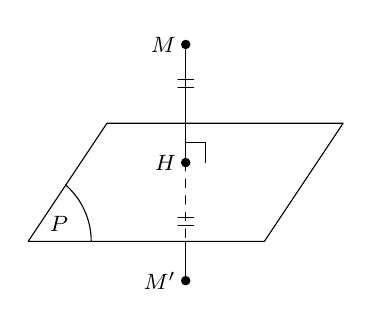
\begin{tikzpicture}[scale=0.5, font=\footnotesize,line join=round, line cap=round, >=stealth]
			\draw (0,0)--(-2,-3)--(4,-3)--(6,0)--cycle;
			\draw (2,2)--(2,-1) (2,-3)--(2,-4);
			\draw (2,-0.5)--(2.5,-0.5)--(2.5,-1);
			\draw (1.8,1.1)--(2.2,1.1) (1.8,0.9)--(2.2,0.9);
			\draw (1.8,-2.4)--(2.2,-2.4) (1.8,-2.6)--(2.2,-2.6);
			\draw[dashed] (2,-1)--(2,-3);
			\draw (-2+0.3,-3) node[above right] {$P$};
			\draw[fill=black] (2,-4) circle(3pt) node[left] {$M'$};
			\draw[fill=black] (2,2) circle(3pt) node[left] {$M$};
			\draw[fill=black] (2,-1) circle(3pt) node[left] {$H$};
			\draw (-0.4,-3) arc(0:49:1.9);
		\end{tikzpicture}
	\end{center}
	\textbf{Lưu ý: } Để tìm điểm đối xứng $M'$ của điểm $M$ qua $(P) \Rightarrow H$ là trung điểm của $MM'$.
	\textbf{2. Tìm hình chiếu $H$ của điểm $M$ lên đường thẳng $d$}
	Viết phương trình mặt phẳng $(P)$ qua $M$ và vuông góc với $d$, khi đó
	$H = d \cap (P)$ thỏa $\heva{&x=x_0+a_1t\\&y=y_0+a_2t\\&z=z_0+a_3t\\&ax+by+cz+d=0\\} \Rightarrow \heva{&x=?\\&y=?\\&z=?\\} \Rightarrow H$.
	\begin{center}
		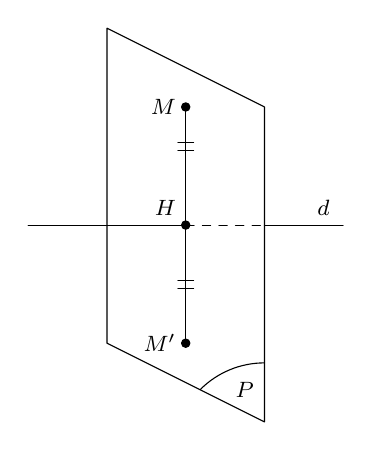
\begin{tikzpicture}[scale=0.5, font=\footnotesize,line join=round, line cap=round, >=stealth]
			\draw (0,4)--(0,-4)--(4,-6)--(4,2)--cycle;
			\draw (2,2)--(2,-4);
			\draw (1.8,1.1)--(2.2,1.1) (1.8,0.9)--(2.2,0.9);
			\draw (1.8,-2.4)--(2.2,-2.4) (1.8,-2.6)--(2.2,-2.6);
			\draw (-2,-1)--(2,-1) (4,-1)--(6,-1);
			\draw[dashed] (2,-1)--(4,-1);
			\draw (4-0.5,-6+0.8) node {$P$};
			\draw (4,-4.5) arc(90:135:2.3);
			\draw[fill=black] (2,-4) circle(3pt) node[left] {$M'$};
			\draw[fill=black] (2,2) circle(3pt) node[left] {$M$};
			\draw[fill=black] (2,-1) circle(3pt) node[above left] {$H$};
			\draw[fill=black] (5.5,-1) node[above] {$d$};
		\end{tikzpicture}
	\end{center}
	\textbf{Lưu ý: } Để tìm điểm đối xứng $M'$ của điểm $M$ qua $d \Rightarrow H$ là trung điểm của $MM'$.
\end{dang}
\Opensolutionfile{ans}[ans/ans-2-C5B2CD3-D3-TN]
%Cau-61
\begin{ex}%[2H5H2-6]
	Trong không gian $Oxyz$, khoảng cách từ điểm $M\left(2; -4; -1\right)$ tới đường thẳng $\Delta \colon \heva{
		& x=t \\ 
		& y=2-t \\ 
		& z=3+2t \\ 
	}$ bằng
	\choice
	{$\sqrt{14}$}
	{$\sqrt{6}$}
	{\True $2\sqrt{14}$}
	{$2\sqrt{6}$}
	\loigiai{
		Đường thẳng $\Delta $ đi qua $N\left(0; 2; 3\right)$, có véc-tơ chỉ phương $\overrightarrow{u}=\left(1; -1; 2\right)$.\\
		$\overrightarrow{MN}=\left(-2;6;4\right);\ \left[\overrightarrow{MN},\overrightarrow{u}\right]=\left(16;8;-4\right)$.\\
		$\mathrm{d}\left(M,\Delta \right)=\dfrac{\left| \left[ \overrightarrow{MN},\overrightarrow{u} \right] \right|}{\left| \overrightarrow{u} \right|}=\dfrac{\sqrt{336}}{\sqrt{6}}=2\sqrt{14}.$
	}
\end{ex}
%Cau-62
\begin{ex}%[2H5V2-6]
	Trong không gian $Oxyz$, tọa độ hình chiếu vuông góc của $M\left(1;0;1 \right)$ lên đường thẳng $\left( \Delta  \right) \colon \dfrac{x}{1}=\dfrac{y}{2}=\dfrac{z}{3}$ là
	\choice
	{$\left( 2;4;6 \right)$}
	{$\left( 1;\dfrac{1}{2};\dfrac{1}{3} \right)$}
	{$\left( 0;0;0 \right)$}
	{\True $\left( \dfrac{2}{7};\dfrac{4}{7};\dfrac{6}{7} \right)$}
	\loigiai{
		Đường thẳng $\Delta $ có véc-tơ chỉ phương $\overrightarrow{u}=\left( 1;2;3 \right)$ và có phương trình tham số là $\heva{
			x=t  \\
			y=2t  \\
			z=3t  \\
		}\left( t\in \mathbb{R} \right)$.\\
		Gọi $N\left( t;2t;3t \right)\in \Delta $ là hình chiếu vuông góc của $M$ lên $\Delta $, khi đó\\
		$\overrightarrow{MN} \cdot \overrightarrow{u}=0\Leftrightarrow (t-1)+(2t-0)\cdot 2+(3t-1)\cdot 3=0\Leftrightarrow 14t-4=0\Leftrightarrow t=\dfrac{2}{7}\Rightarrow N\left( \dfrac{2}{7};\dfrac{4}{7};\dfrac{6}{7} \right)$.
	}
\end{ex}
%Cau-63
\begin{ex}%[2H5V2-6]
	Trong không gian với hệ tọa độ $Oxyz$, cho điểm $M(-4;0;0)$ và đường thẳng $\Delta \colon \heva{
		& x=1-t \\ 
		& y=-2+3t \\ 
		& z=-2t \\ 
	}$. Gọi $H(a;b;c)$ là hình chiếu của $M$ lên $\Delta $. Tính $a+b+c$.
	\choice
	{$5$}
	{\True $-1$}
	{$-3$}
	{$7$}
	\loigiai{
		Gọi $H$ là hình chiếu của $M$ lên $\Delta $ nên tọa độ của $H$ có dạng $H(1-t;-2+3t;-2t)$ và $\overrightarrow{MH}\perp \overrightarrow{u}_{\Delta}$.\\
		$\Rightarrow \overrightarrow{MH} \cdot \overrightarrow{u}_{\Delta }=0\Leftrightarrow 14t-11=0\Leftrightarrow t=\dfrac{11}{14}\Rightarrow H\left(\dfrac{3}{14};\dfrac{5}{14};\dfrac{-22}{14}\right)\Rightarrow a+b+c=-1$.
	}
\end{ex}
%Cau-64
\begin{ex}%[2H5V2-4]
	Trong không gian $Oxyz$, tọa độ hình chiếu vuông góc của điểm $A\left( 3;2;-1 \right)$ lên mặt phẳng $\left( \alpha  \right)\colon x+y+z=0$ là
	\choice
	{$\left( -2;1;1 \right)$}
	{\True $\left( \dfrac{5}{3};\dfrac{2}{3};-\dfrac{7}{3} \right)$}
	{$\left( 1;1;-2 \right)$}
	{$\left( \dfrac{1}{2};\dfrac{1}{4};\dfrac{1}{4} \right)$}
	\loigiai{
		Gọi $H$ là hình chiếu của $A\left( 3;2;-1 \right)$ lên mặt phẳng $\left( \alpha  \right)\colon x+y+z=0$. Khi đó $AH$ nhận $\overrightarrow{n}=\left( 1;1;1 \right)$ là vectơ chỉ phương.\\
		Suy ra phương trình $AH \colon \dfrac{x-3}{1}=\dfrac{y-2}{1}=\dfrac{z+1}{1}$.\\
		Do $H\in AH\Rightarrow H\left( 3+t;2+t;-1+t \right)$.\\
		Do $H\in \left( \alpha  \right)\Rightarrow 3+t+2+t-1+t=0\Leftrightarrow t=-\dfrac{4}{3}\Rightarrow H\left( \dfrac{5}{3};\dfrac{2}{3};-\dfrac{7}{3} \right)$.
	}
\end{ex}
%Cau-65
\begin{ex}%[2H5V2-5]
	Trong không gian với hệ trục tọa độ $Oxyz$, hình chiếu của điểm $M\left( -1;0;3 \right)$ theo phương vectơ $\overrightarrow{v}=\left( 1;-2;1 \right)$ trên mặt phẳng $\left( P \right) \colon x-y+z+2=0$ có tọa độ là
	\choice
	{$\left( 2;-2;-2 \right)$}
	{$\left( -1;0;1 \right)$}
	{\True $\left( -2;2;2 \right)$}
	{$\left( 1;0;-1 \right)$}
	\loigiai{
		\begin{center}
			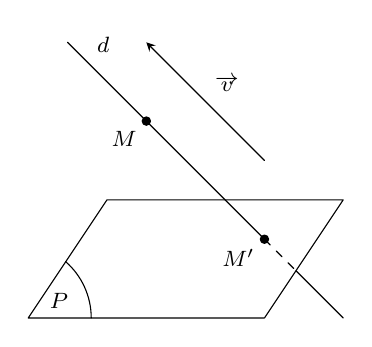
\begin{tikzpicture}[scale=0.5, font=\footnotesize,line join=round, line cap=round, >=stealth]
				\draw (0,0)--(-2,-3)--(4,-3)--(6,0)--cycle;
				\draw (-1,4)--(4,-1) (4.8,-1.8)--(6,-3);
				\draw[dashed] (4,-1)--(4.8,-1.8);
				\draw[->] (4,1)--(1,4);
				\draw (-2+0.3,-3) node[above right] {$P$};
				\draw[fill=black] (4,-1) circle(3pt) node[below left] {$M'$};
				\draw[fill=black] (1,2) circle(3pt) node[below left] {$M$};
				\draw (-0.5,3.5) node[above right] {$d$};
				\draw (2.5,2.5) node[above right] {$\overrightarrow{v}$};
				\draw (-0.4,-3) arc(0:49:1.9);
			\end{tikzpicture}
		\end{center}
		Đường thẳng $d$ đi qua $M\left( -1;0;3 \right)$, có véc-tơ chỉ phương $\overrightarrow{v}=\left( 1;-2;1 \right)$ có phương trình tham số là $\heva{
			& x=-1+t \\ 
			& y=-2t \\ 
			& z=3+t. \\ 
		}$\\
		Gọi $M'$ là hình chiếu của điểm $M\left( -1;0;3 \right)$ theo phương véc-tơ $\overrightarrow{v}=\left( 1;-2;1 \right)$ trên mặt phẳng $\left( P \right) \colon x-y+z+2=0$.\\
		$\Rightarrow M'=d\cap \left( P \right)\Rightarrow $ tọa độ $M'$ là nghiệm của hệ phương trình\\
		$\heva{
			& x=-1+t \\ 
			& y=-2t \\ 
			& z=3+t \\ 
			& x-y+z+2=0 \\ 
		}\Leftrightarrow \heva{
			& x=-1+t \\ 
			& y=-2t \\ 
			& z=3+t \\ 
			& -1+t+2t+3+t+2=0 \\ 
		}\Leftrightarrow \heva{
			& x=-2 \\ 
			& y=2 \\ 
			& z=2 \\ 
			& t=-1 \\ 
		}\Rightarrow M'\left( -2;2;2 \right)$.
		
	}
\end{ex}
%Cau-66
\begin{ex}%[2H5V2-5]
	Trong không gian với hệ tọa độ $Oxyz$, cho mặt phẳng $\left( P \right) \colon 6x-2y+z-35=0$ và điểm $A\left( -1;3;6 \right).$ Gọi $A'$ là điểm đối xứng với $A$ qua $\left( P \right)$, tính $OA'.$
	\choice
	{$OA'=5\sqrt{3}$}
	{$OA'=\sqrt{46}$}
	{\True $OA'=\sqrt{186}$}
	{$OA'=3\sqrt{26}$}
	\loigiai{
		$A'$ đối xứng với $A$ qua $\left( P \right)$ nên $AA'$ vuông góc với $\left( P \right)$.\\
		Suy ra phương trình đường thẳng $AA' \colon \heva{
			& x=-1+6t \\ 
			& y=3-2t \\ 
			& z=6+t. \\ 
		}$\\
		Gọi $H$ là giao điểm của $AA'$ và mặt phẳng $\left( P \right) \Rightarrow H\left( -1+6t;3-2t;6+t \right)$.\\
		Do $H$ thuộc $\left( P \right) \Rightarrow 6\left( -1+6t \right)-2\left( 3-2t \right)+1\left( 6+t \right)-35=0 $.\\
		$\Leftrightarrow 41t-41=0\Leftrightarrow t=1\Rightarrow H\left( 5;1;7 \right)$.\\
		$A'$ đối xứng với $A$ qua $\left( P \right)$ nên $H$ là trung điểm của $AA'\Rightarrow {A}'\left( 11;-1;8 \right)\Rightarrow OA'=\sqrt{11^2+\left( -1 \right)^2+8^2}=\sqrt{186}$.
	}
\end{ex}
%Cau-67
\begin{ex}%[2H5V2-2]
	Trong không gian với hệ tọa độ $Oxyz$, cho đường thẳng $d \colon \dfrac{x-1}{1} = \dfrac{y-1}{2} = \dfrac{z-2}{-1}$ và mặt phẳng $(P) \colon 2x+y+2z-1=0$. Gọi $d'$ là hình chiếu của đường thẳng $d$ lên mặt phẳng $(P)$, véc-tơ  chỉ phương của đường thẳng $d'$ là
	\choice
	{$\overrightarrow{u}_3 = (5;-6;-13)$}
	{$\overrightarrow{u}_2 = (5;-4;-3)$}
	{$\overrightarrow{u}_4 = (5;16;13)$}
	{\True $\overrightarrow{u}_1 = (5;16;-13)$}
	\loigiai{
		Đường thẳng $d$ đi qua điểm $A(1;1;2)$ và có một véc-tơ chỉ phương $\overrightarrow{u}_d = (1;2;-1)$.\\
		Mặt phẳng $(P)$ có một véc-tơ pháp tuyến $\overrightarrow{n}_{(P)}= (2;1;2)$.\\
		Gọi $\overrightarrow{u}_{d'}$ là một  véc-tơ chỉ phương của đường thẳng $d'$.\\
		Gọi $(Q)$ là mặt phẳng chứa đường thẳng $d$ và vuông góc với mặt phẳng $(P)$. Khi đó, $(Q)$ đi qua điểm $A(1;1;2)$ và có một véc-tơ pháp tuyến $\overrightarrow{n}_{(Q)} = \left[\overrightarrow{u}_d, \overrightarrow{u}_{(P)}\right] = (5;-4;-3)$.\\
		Đường thẳng $d'$ là hình chiếu của đường thẳng $d$ trên mặt phẳng $(P) \Leftrightarrow d' = (P) \cap (Q)$ nên  $\heva{&\overrightarrow{u}_{d'} \perp \overrightarrow{n}_{(P)}\\&\overrightarrow{u}_{d'} \perp \overrightarrow{n}_{(Q)}.}$\\
		Véc-tơ chỉ phương của đường thẳng $d'$ là $\overrightarrow{u}_{d'}=\left[\overrightarrow{n}_{(P)}, \overrightarrow{n}_{(Q)}\right] =(5;16;-13)$.
	}
\end{ex}
%Cau-68
\begin{ex}%[2H5V2-3]
	Trong không gian $Oxyz$, cho mặt phẳng $(\alpha) \colon 2x+y+z-3=0$ và đường thẳng $d\colon \dfrac{x+4}{3} = \dfrac{y-3}{-6} = \dfrac{z-2}{-1}$. Viết phương trình đường thẳng $d'$ đối xứng với đường thẳng $d$ qua mặt phẳng $(\alpha)$.
	\choice
	{$\dfrac{x}{11} = \dfrac{y+5}{-17} = \dfrac{z-4}{-2}$}
	{$\dfrac{x}{11} = \dfrac{y-5}{-17} = \dfrac{z+4}{-2}$}
	{\True $\dfrac{x}{11} = \dfrac{y-5}{-17} = \dfrac{z-4}{-2}$}
	{$\dfrac{x}{11} = \dfrac{y-5}{-17} = \dfrac{z-4}{2}$}
	\loigiai{
		Mặt phẳng $(\alpha) \colon 2x+y+z-3=0$ có véc-tơ pháp tuyến là $\overrightarrow{n} = (2;1;1)$.\\
		Gọi tọa độ giao điểm của $d$ và $(\alpha)$ là $I$ thì $I(-22;39;8)$.\\
		Lấy $A(-4;3;2) \in d$. Gọi $\Delta$ là đường thẳng đi qua $A$ và vuông góc với $(\alpha)$.\\
		Suy ra phương trình đường thẳng $\Delta \colon \heva{&x=-4+2t\\&y=3+t\\&z=2+t.\\}$\\
		Gọi $H$ là hình chiếu của $A$ lên $(\alpha)$ thì $H = \Delta \cap (\alpha)\Rightarrow H(-2;4;3)$.\\
		$A'$ đối xứng với $A$ qua $(\alpha) \Leftrightarrow H$ là trung điểm của $AA'$, $d'$ có véc-tơ chỉ phương $\overrightarrow{A'I} = (22;-34;-4) = 2(11;-17;-2)$ có phương trình là $\dfrac{x}{11} = \dfrac{y-5}{-17} = \dfrac{z-4}{-2}$.
	}
\end{ex}
%Cau-69
\begin{ex}%[2H5C2-3]
	Trong không gian $Oxyz$, cho đường thẳng $d \colon \dfrac{x-1}{2} = \dfrac{y+5}{-1} = \dfrac{z-3}{4}$. Phương trình nào dưới đây là phương trình hình chiếu vuông góc của $d$ trên mặt phẳng $x+3=0$?
	\choice
	{$\heva{&x=-3\\&y=-5+2t\\&z=3-t\\}$}
	{\True $\heva{&x=-3\\&y=-6-t\\&z=7+4t\\}$}
	{$\heva{&x=-3\\&y=-5-t\\&z=-3+4t\\}$}
	{$\heva{&x=-3\\&y=-5+t\\&z=3+4t\\}$}
	\loigiai{
		Đường thẳng $d$ đi qua điểm $M_0(1;-5;3)$ và có véc-tơ chỉ phương $\overrightarrow{u}_d=(2;-1;4)$.\\
		Gọi $(Q)$ là mặt phẳng chứa $d$ và vuông góc với $(P) \colon x + 3 = 0$.\\
		Suy ra mặt phẳng $(Q)$ đi qua điểm $M_0(1;-5;3)$ và có véc-tơ pháp tuyến là $\left[\overrightarrow{n}_{(P)}; \overrightarrow{u}_d\right] = (0;4;1)$.\\
		$\Rightarrow (Q) \colon 4y+z+17=0$.\\
		Phương trình hình chiếu của $d$ lên mặt phẳng $(P)$ là \\
		$$\heva{&4y+z+17=0\\&x+3=0} \text{hay} \heva{&x=-3\\&y=-6-t\\&z=7+4t.}$$\\
	}
\end{ex}
%Cau-70
\begin{ex}%[2H5C2-3]
	Trong không gian $Oxyz$, cho mặt phẳng $(P) \colon x+y+z-3=0$ và đường thẳng $d \colon \dfrac{x}{1} = \dfrac{y+1}{2} = \dfrac{z-2}{-1}$. Hình chiếu vuông góc của $d$ trên $(P)$ có phương trình là
	\choice
	{\True $\dfrac{x-1}{1} = \dfrac{y-1}{4} = \dfrac{z-1}{-5}$}
	{$\dfrac{x-1}{1} = \dfrac{y-1}{4} = \dfrac{z+5}{1}$}
	{$\dfrac{x+1}{-1} = \dfrac{y+1}{-4} = \dfrac{z+1}{5}$}
	{$\dfrac{x-1}{3} = \dfrac{y-1}{-2} = \dfrac{z-1}{-1}$}
	\loigiai{
		Gọi $M$ là giao điểm của $d$ và $(P)$.\\
		Tọa độ của $M$ là nghiệm của hệ $$\heva{&x+y+z-3=0\\&\dfrac{x}{1} = \dfrac{y+1}{2} = \dfrac{z-2}{-1}\\} \Leftrightarrow \heva{&x+y+z=3\\&2x-y=1\\&x+z=2\\}\Leftrightarrow \heva{&x=1\\&y=1\\&z=1\\} \Rightarrow M(1;1;1).$$
		Lấy điểm $N(0;-1;2) \in d$.\\
		Một véc-tơ pháp tuyến của mặt phẳng $(P)$ là $\overrightarrow{n} = (1;1;1)$.\\
		Gọi $\Delta$ là đường thẳng đi qua $N$ và nhận $\overrightarrow{n}=(1;1;1)$ làm véc-tơ chỉ phương.\\
		Phương trình đường thẳng $\Delta \colon \dfrac{x}{1} = \dfrac{y+1}{1} = \dfrac{z-2}{1}$.\\
		Gọi $N'$ là giao điểm của $\Delta$ với $(P)$.\\
		Tọa độ của $N'$ là nghiệm của hệ
		$$\heva{&x+y+z-3=0\\&\dfrac{x}{1} = \dfrac{y+1}{1} = \dfrac{z-2}{1}\\} \Leftrightarrow \heva{&x+y+z=3\\&x-y=1\\&x-z=-2\\} \Leftrightarrow \heva{&x=\dfrac{2}{3}\\&y=-\dfrac{1}{3}\\&z=\dfrac{8}{3}} \Rightarrow N'\left(\dfrac{2}{3};-\dfrac{1}{8};\dfrac{8}{3}\right).$$
		$\overrightarrow{MN'} = \left(-\dfrac{1}{3};-\dfrac{4}{3};\dfrac{5}{3}\right) = -\dfrac{1}{3}(1;4;-5)$.\\
		Đường thẳng cần tìm đi qua điểm $M(1;1;1)$ và nhận $\overrightarrow{u} = (1;4;-5)$ làm véc-tơ chỉ phương nên có phương trình $\dfrac{x-1}{1} = \dfrac{y-1}{4} = \dfrac{z-1}{-5}$.
	}
\end{ex}
%Cau-71
\begin{ex}%[2H5C2-3]
	Trong không gian với hệ tọa độ $Oxyz$, cho mặt phẳng $(P) \colon x+y-z-1=0$ và đường thẳng $d \colon \dfrac{x+2}{2} = \dfrac{y-4}{-2} = \dfrac{z+1}{1}$. Viết phương trình đường thẳng $d'$ là hình chiếu vuông góc của $d$ lên $(P)$.
	\choice
	{$d' \colon \dfrac{x+2}{7} = \dfrac{y}{-5} = \dfrac{z+1}{2}$}
	{\True $d' \colon \dfrac{x-2}{7} = \dfrac{y}{-5} = \dfrac{z-1}{2}$}
	{$d' \colon \dfrac{x+2}{7} = \dfrac{y}{5} = \dfrac{z+1}{2}$}
	{$d' \colon \dfrac{x-2}{7} = \dfrac{y}{5} = \dfrac{z-1}{2}$}
	\loigiai{
		Phương trình tham số của $d \colon \heva{&x=-2+2t\\&y=4-2t\\&z=-1+t\\}, \ t \in \mathbb{R}$. \\
		Gọi $M = (-2+2t;4-2t;-1+t)$  là giao điểm của $d$ và $(P)$.\\
		$\Rightarrow (-2+2t) + (4-2t) - (-1+t) - 1 = 0 \Leftrightarrow t = 2 \Rightarrow M=( 2;0;1)$.\\
		Mặt phẳng $(P)$ có một véc-tơ pháp tuyến là $\overrightarrow{n}_{(P)} = (1;1;-1)$. Điểm $N = (0;2;0) \in d$.\\
		Gọi $\Delta$ là đường thẳng đi qua $N(0;2;0)$ và vuông góc với mặt phẳng $(P) \Rightarrow \Delta$ nhận $\overrightarrow{n}_{(P)} = (1;1;-1)$ làm véc-tơ chỉ phương. Suy ra phương trình của $\Delta$ là
		$$\Delta \colon \dfrac{x-0}{1} = \dfrac{y-2}{1} = \dfrac{z-0}{-1} \Leftrightarrow \Delta \colon \heva{&x=c\\&y=2+c\\&z=-c\\}, \ c \in \mathbb{R}.$$
		Gọi $M'=(c;2+c;-c)$ là giao điểm của $\Delta$  với mặt phẳng $(P) \Rightarrow c+(2+c)-(-c)-1=0 \Leftrightarrow c=-\dfrac{1}{3} \Rightarrow M'\left(-\dfrac{1}{3};\dfrac{5}{3};\dfrac{1}{3}\right)$.\\
		$\overrightarrow{MM'}=\left(-\dfrac{7}{3};\dfrac{5}{3};-\dfrac{2}{3}\right)$, đường thẳng $d'$ là hình chiếu vuông góc của $d$ trên mặt phẳng $(P)$ nên $d'$ chính là đường thẳng $MM'$, suy ra $d'$ đi qua $M(2;0;1)$ và nhận véc-tơ $\overrightarrow{u} = -3\overrightarrow{MM'}=(7;-5;2)$ làm véc-tơ chỉ phương nên phương trình của $d'$ là\\
		$d' \colon \dfrac{x-2}{7} = \dfrac{y}{-5} = \dfrac{z-1}{2}$.
	}
\end{ex}
\begin{ex}%[2H5V2-3]
	Trong không gian với hệ tọa độ $Oxyz$, cho mặt phẳng $(P)\colon x+y-z-1=0$ và đường thẳng $d\colon \dfrac{x+2}{2}=\dfrac{y-4}{-2}=\dfrac{z+1}{1}$. Viết phương trình đường thẳng $d'$ là hình chiếu vuông góc của $d$ trên $(P)$.
	\choice
	{$d'\colon \dfrac{x+2}{7}=\dfrac{y}{-5}=\dfrac{z+1}{2}$}
	{\True $d'\colon \dfrac{x-2}{7}=\dfrac{y}{-5}=\dfrac{z-1}{2}$}
	{$d'\colon \dfrac{x+2}{7}=\dfrac{y}{5}=\dfrac{z+1}{2}$}
	{$d'\colon \dfrac{x-2}{7}=\dfrac{y}{5}=\dfrac{z-1}{2}$}
	\loigiai{
		$(\Delta)\colon \dfrac{x-0}{1}=\dfrac{y-2}{1}=\dfrac{z-0}{-1} \Leftrightarrow(\Delta)\colon \heva{&x=c \\& y=2+c\\& z=-c}$, $c\in \mathbb{R}$.\\
		Gọi $M'=(c;2+c;-c)$ là giao điểm của $\Delta$ với mặt phẳng $(P)$. Lúc đó $$c+(2+c)-(-c)-1=0 \Leftrightarrow c=-\dfrac{1}{3}.$$
		Suy ra $M'\left(-\dfrac{1}{3};\dfrac{5}{3}; \dfrac{1}{3}\right)$, $\overrightarrow{MM'}=\left(-\dfrac{7}{3}; \dfrac{5}{3};-\dfrac{2}{3}\right)$. \\
		Đường thẳng $d'$ là hình chiếu vuông góc của $d$ trên mặt phẳng $(P)$ nên $d'$ chính là đường thẳng $MM'$.\\
		Vậy $d'$ đi qua $M(2;0;1)$ và nhận vectơ $\vec{u}=-3\overrightarrow{MM'}=(7 ;-5;2)$ làm vectơ chỉ phương nên phương trình của $d'$ là $d'\colon \dfrac{x-2}{7}=\dfrac{y}{-5}=\dfrac{z-1}{2}$.
	}
\end{ex}
\begin{ex}%[2H5V2-3]
	Trong không gian với hệ tọa độ $Oxyz$, cho mặt phẳng $(\alpha)\colon x+y-z+6=0$ và đường thẳng $d\colon\dfrac{x-1}{2}=\dfrac{y+4}{3}=\dfrac{z}{5}$. Hình chiếu vuông góc của $d$ trên $(\alpha)$ có phương trình là
	\choice 										      
	{$\dfrac{x+1}{2}=\dfrac{y+4}{3}=\dfrac{z-1}{5}$}
	{\True $\dfrac{x}{2}=\dfrac{y+5}{3}=\dfrac{z-1}{5}$}
	{$\dfrac{x+5}{2}=\dfrac{y}{3}=\dfrac{z-1}{5}$}
	{$\dfrac{x}{2}=\dfrac{y-5}{3}=\dfrac{z-1}{5}$}
	\loigiai{ 
		Mặt phẳng $(\alpha)\colon x+y-z+1=0$ có vectơ pháp tuyến $\vec{n}=(1;1;-1)$. \\
		Đường thẳng $d\colon \dfrac{x-1}{2}=\dfrac{y+4}{3}=\dfrac{z}{5}$ có vectơ chỉ phương $\vec{u}=(2;3;5)$.\\
		Vì $\vec{n} \cdot \vec{u}=1 \cdot 2+1.3+(-1) \cdot 5=0$ nên $d\parallel (\alpha)$.\\
		Gọi $d'$ là hình chiếu vuông góc của $d$ trên $(\alpha)$. Lúc đó $d'\parallel d$.\\
		Lấy $A(1;-4;0) \in d$. Gọi $\Delta$ là đường thẳng đi qua $A$ và vuông góc với $(\alpha)$. Suy ra phương trình đường thẳng $\Delta$ là $\heva{&x=1+t \\ &y=-4+t \\ &z=-t.}$\\
		Gọi $A'$ là hình chiếu của $A$ lên $(\alpha)$ thì $A'=\Delta \cap(\alpha) \Rightarrow A'(0;-5;1)$.\\
		Đường thẳng $d'$ là đường thẳng đi qua $A'(0;-5;1)$, có vectơ chỉ phương $\vec{u}=(2;3;5)$ có phương trình là $\dfrac{x}{2}=\dfrac{y+5}{3}=\dfrac{z-1}{5}$.
	}
\end{ex}


\begin{ex}%[2H5V2-3]
	Trong không gian với hệ tọa độ $Oxyz$, cho mặt phẳng $(P)\colon x+y+z-3=0$ và đường thẳng $d\colon \dfrac{x}{1}=\dfrac{y+1}{2}=\dfrac{z-2}{-1}$. Hình chiếu của $d$ trên $(P)$ có phương trình là đường thẳng $d'$. Trong các điểm sau điểm nào thuộc đường thẳng $d'$?
	\choice 
	{\True $M(2;5;-4)$}
	{$P(1;3;-1)$}
	{$N(1;-1;3)$}
	{$Q(2;7;-6)$}
	\loigiai{
		Gọi  $A=d \cap (P)$. Vì $A \in d\colon \heva{&	x=t\\&y=-1+2t\\&z=2-t} \Rightarrow A(t;-1+2t;2-t)$.\\
		Mặt khác $A \in (P) \Rightarrow t-1+2 t+2-t-3=0 \Leftrightarrow t=1$. Vậy $A(1; 1;1)$.\\
		Lấy $B(0;-1;2)\in d$. Gọi $\Delta$ là đường thẳng qua $B$ và vuông góc $(P)$ thì $\Delta\colon\heva{&x=t'\\&y=-1+t'\\&z=2+t'.}$\\
		Gọi $C$ là hình chiếu của $B$ lên $(P)$. Ta có $C \in \Delta \Rightarrow C\left(t';-1+t';2+t'\right)$.\\
		Mặt khác $C \in(P) \Rightarrow t'-1+t'+2+t'-3=0 \Leftrightarrow t'=\dfrac{2}{3}$.\\
		Vậy 
		$C\left(\dfrac{2}{3};\dfrac{-1}{3};\dfrac{8}{3}\right)$.\\
		Lúc này $d'$ qua $A(1;1;1)$ và có một vectơ chỉ phương là $\overrightarrow{AC}=\left(-\dfrac{1}{3};-\dfrac{4}{3};\dfrac{5}{3}\right)$. Hay $d'$ nhận $\vec{u}=(1;4;-5)$ làm một vectơ chỉ phương.\\
		Suy ra $d'\colon\heva{&x=1+s \\ &y=1+4 s \\ &z=1-5 s.}$ \\
		Vậy điểm thuộc đường thẳng $d'$ là $M(2;5;-4)$.
	}
\end{ex}

\begin{ex}%[2H5V2-3]
	Trong không gian với hệ tọa độ $Oxyz$, cho đường thẳng $d\colon \dfrac{x-1}{2}=\dfrac{y-2}{1}=\dfrac{z+1}{3}$ và mặt phẳng $(P)\colon x+y+z-3=0$. Đường thẳng $d'$ là hình chiếu của $d$ theo phương $Ox$ lên $(P)$, $d'$ nhận $\vec{u}=(a;b;2019)$ làm một vectơ chỉ phương. Xác định tổng $a+b$.
	\choice 
	{$2019$}
	{\True $-2019$}
	{$2018$}
	{$-2020$}
	\loigiai{
		\begin{center}
			\begin{tikzpicture}[scale=2]
				\def\a{3}
				\def\b{1}
				\def\g{30}
				\def\h{2}
				\path
				(0:0) coordinate (A)--++(\g:\b) coordinate (B)--++(0:\a) coordinate (C)--++(\g-180:\b) coordinate (D)--++(\g+143:2.1) coordinate (E)--++(0:.3) coordinate (F)--++(0:1.7) coordinate (G)--++(0:.2) coordinate (H)--++(150:2) coordinate (M)--++(150:.3) coordinate (N)--++(-20:2)coordinate (O);
				\draw  pic [draw, angle radius = 10 mm,"$P$"] {angle = D--A--B}; 		
				\coordinate (I) at ($(M)!1.2!(F)$);
				\coordinate (J) at ($(F)!1.3!(M)$);
				\coordinate (K) at ($(N)!1.1!(G)$);
				\coordinate[label = right:$x$] (P) at ($(J)+(O)-(F)$); 
				\coordinate (Q) at ($(P)!1.1!(O)$);	
				\draw
				(A)--(B)--(C)--(D)--cycle (Q)--(P)  (H)--(E) node [left]{$d'$} (N) node[left]{$d$}--(G)node[below]{$A$} (F) node[below right]{$H$}--(J);
				\draw[dashed](I)--(F)(K)--(G);
				\fill (F) circle (1pt) (G) circle (1pt) (M) node[above right]{$M$} circle (1pt) (O) node[right]{$O$} circle (1pt);
			\end{tikzpicture}
		\end{center}
		Mặt phẳng $(P)$ có vectơ pháp tuyến là $\vec{n}_{(P)}=(1;1;1)$, đường thẳng $d$ có vectơ chỉ phương là $\vec{u}_d=(2;1;3)$, đường thẳng chứa trục  $Ox$ có vectơ chỉ phương $\vec{i}=(1;0;0)$.\\
		Gọi $(Q)$ là mặt phẳng chứa đường thẳng $d$ và song song (hoặc chứa) trục $Ox$. Khi đó $(Q)$ có vectơ pháp tuyến $\vec{n}_{(Q)}=\left[\vec{u}_d, \vec{i}\right]=(0;3;-1)$.\\
		Đường thẳng $d'$ chính là giao tuyến của $(P)$ và $(Q)$. Từ đó có vectơ chỉ phương của $d'$ là $\vec{u}_1=\left[\vec{n}_{(P)}, \vec{n}_{(Q)}\right]=(-4;1;3)$.\\
		Suy ra $\vec{u}=(-2692;673;2019)$ cũng là vectơ chỉ phương của $d'$.\\ Ta có $a+b=-2692+673=-2019$.
	}
\end{ex}

\begin{ex}%[2H5V2-3]
	Trong không gian với hệ tọa độ $Oxyz$, cho hai đường thẳng $d\colon \heva{&x=-2\\& y=t\\&z=2+2t}$, $(t \in \mathbb{R})$, $\Delta\colon\dfrac{x-3}{1}=\dfrac{y-1}{-1}=\dfrac{z-4}{1}$ và mặt phẳng $(P)\colon x+y-z+2=0$. Gọi $d'$ và $\Delta'$ lần lượt là hình chiếu của $d$ và $\Delta$ lên mặt phẳng $(P)$. Gọi $M(a;b;c)$ là giao điểm của hai đường thẳng $d'$ và $\Delta'$. Biểu thức $a+b\cdot c$ bằng
	\choice 
	{$4$}
	{\True $5$}
	{$3$}
	{$6$}
	\loigiai{
		Do $d'$ là hình chiếu của $d$ lên mặt phẳng $(P)$ nên $d'$ là giao tuyến của mặt phẳng $(P)$ và mặt phẳng $(\alpha)$ chứa $d$ và vuông góc với mặt phẳng $(P)$. Suy ra một vectơ pháp tuyến của mặt phẳng $(\alpha)$ là $\vec{n}_{(\alpha)}=\left[\vec{u_d}, \vec{n}_{P}\right]=(-3;2;-1)$.\\
		Mặt phẳng $(\alpha)$ đi qua $A(-2;0;2)$ và có một vectơ pháp tuyến $\vec{n}_{(\alpha)}=(-3;2;-1)$ có phương trình là $$3x-2y+z+4=0.$$
		Do $\Delta'$ là hình chiếu của $\Delta$ lên mặt phẳng $(P)$ khi đó $\Delta'$ là giao tuyến của mặt phẳng $(P)$ và mặt phẳng $(\beta)$ chứa $\Delta$ và vuông góc vởi mặt phẳng $(P)$. Suy ra  một vectơ pháp tuyến của mặt phẳng $(\beta)$ là $\vec{n}_{(\beta)}=\left[\vec{u}_{\Delta}, \vec{n}_P\right]=(0;-2;-2)$.\\
		Mặt phẳng $(\beta)$ đi qua $B(3;1;4)$ và có một vectơ pháp tuyến
		$\vec{n}_{(\beta)}=(0;-2;-2)$ có phương trình là 
		$$y+z-5=0.$$
		Tọa độ điểm $M$ là nghiệm của hệ phương trình $\heva{&x+y-z+2=0 \\&3x-2y+z+4=0 \\&y+z-5=0} \Leftrightarrow\heva{&x=-1 \\ &y=2 \\&z=3.}$\\
		Vậy $M(-1;2;3) \Rightarrow a+b \cdot c=-1+2 \cdot 3=5$.
	}
\end{ex}

\begin{ex}%[2H5V2-3]
	Trong không gian với hệ tọa độ $Oxyz$, cho điểm  $A(1;1;1)$ và đường thẳng $d\colon\heva{&x=1+t \\& y=1+t \\&z=t}$. Tìm tọa độ điểm $H$ là hình chiếu của $A$ lên đường thẳng $\Delta$.
	\choice 
	{\True $H\left(\dfrac{4}{3};\dfrac{4}{3};\dfrac{1}{3}\right)$}
	{$H(1;1;1)$}
	{$H(0;0;-1)$}
	{$H(1;1;0)$}
	\loigiai{ 
		Đường thẳng $d$ có vectơ chỉ phương là $\overrightarrow{u}=(1;1;1)$.\\
		Do $H \in d \Rightarrow H\left(1+t;1+t;t\right)\Rightarrow\overrightarrow{AH}=(t;t;t-1)$.\\
		Do $H$ là hình chiếu của điểm $A$ lên đường thẳng $d$ nên suy ra $$\overrightarrow{AH} \perp \vec{u} \Leftrightarrow \overrightarrow{AH} \cdot \vec{u}=0 \Leftrightarrow t+t+t-1=0 \Leftrightarrow t=\dfrac{1}{3} \Rightarrow H\left(\dfrac{4}{3};\dfrac{4}{3};1\right).$$
	}
\end{ex}

\begin{ex}%[2H5V2-3]
	Trong không gian với hệ tọa độ $Oxyz$, cho điểm $A(1;1;1)$ và đường thẳng $(d)\colon \heva{&x=6-4t\\&y=-2-t \\&z=-1+2t}$. Tìm tọa độ hình chiếu $A'$ của $A$ trên $(d)$.
	\choice 
	{$A'(2;3;1)$}
	{$A'(-2;3;1)$}
	{\True $A'(2;-3;1)$}
	{$A'(2;-3;-1)$}
	\loigiai{
		Ta có $A'\in(d)$ nên gọi $A'(6-4 t;-2-t;-1+2 t)$, suy ra $\overrightarrow{AA'}=(5-4t;-3-t;-2+2t)$.\\
		Đường thẳng $(d)$ có vectơ chỉ phương $\vec{u}=(-4;-1;2)$.\\
		Vì $AA' \perp (d) \Leftrightarrow \overrightarrow{AA'} \cdot \vec{u}=0 \Leftrightarrow(5-4t) \cdot(-4)+(-3-t) \cdot(-1)+(-2+2 t) \cdot 2=0 \Leftrightarrow t=1$. Vậy $A'(2 ;-3 ; 1)$.
	}
\end{ex}

\begin{ex}%[2H5V2-3]
	Trong không gian với hệ tọa độ $Oxyz$, cho đường thẳng $d\colon \dfrac{x+1}{1}=\dfrac{y+3}{2}=\dfrac{z+2}{2}$ và điểm $A(3;2;0)$. Điểm đối xứng của điểm $A$ qua đường thẳng $d$ có tọa độ là
	\choice 
	{\True $(-1;0;4)$}
	{$(7;1;-1)$}
	{$(2;1;-2)$}
	{$(0;2;-5)$}
	\loigiai{
		Gọi $(P)$ là mặt phẳng đi qua $A$ và vuông góc với đường thẳng $d$. Phương trình của mặt phẳng $(P)$ là $1(x-3)+2(y-2)+2(z-0)=0$ $\Leftrightarrow x+2 y+2 z-7=0$.\\
		Gọi $H$ là hình chiếu của $A$ lên đường thẳng $d$, khi đó $H=d \cap (P)$.\\
		Vì $H \in d$ nên $ H(-1+t ;-3+2 t ;-2+2 t)$.\\
		Mặt khác $H \in(P) $ nên $-1+t-6+4 t-4+4 t-7=0 \Rightarrow t=2$.\\ Vậy $H(1;1;2)$.\\
		Gọi $A'$ là điểm đối xứng với $A$ qua đường thẳng $d$, khi đó $H$ là trung điểm của $AA'$.\\
		Suy ra $A'(-1;0;4)$.
	}
\end{ex}

\begin{ex}%[2H5V2-3]
	Trong không gian với hệ tọa độ $Oxyz$, xác định tọa độ điểm $M'$ là hình chiếu vuông góc của điểm $M(2;3;1)$ lên mặt phẳng $(\alpha)\colon x-2y+z=0$.
	\choice
	{$M'\left(2;\dfrac{5}{2};3\right)$}
	{$M'(1;3;5)$}
	{\True  $M'\left(\dfrac{5}{2};2;\dfrac{3}{2}\right)$}
	{$M'(3;1;2)$}
	\loigiai{
		Gọi $\Delta$ là đường thẳng qua $M$ và vuông góc với $(\alpha)$.\\ Phương trình tham số của $\Delta$ là $\heva{&x=2+t \\ &y=3-2 t \\& z=1+t}$. Ta có $M'=\Delta \cap(\alpha)$.\\
		Xét phương trình $2+t-2(3-2t)+1+t=0 \Leftrightarrow t=\dfrac{1}{2}$.\\
		Vậy $M'\left(\dfrac{5}{2};2;\dfrac{3}{2}\right)$.
	}
\end{ex}

\begin{ex}%[2H5V1-3]
	Trong không gian với hệ trục tọa độ $Oxyz$, điểm $M'$ đối xứng với điểm $M(1;2;4)$ qua mặt phẳng $(\alpha)\colon 2x+y+2z-3=0$ có tọa độ là
	\choice
	{\True $(-3;0;0)$}
	{$(-1;1;2)$}
	{$(-1 ;-2 ;-4)$}
	{$(2;1;2)$}
	\loigiai{
		Mặt phẳng $(\alpha)$ có vectơ pháp tuyến là $\vec{n}=(2;1;2)$.\\
		Vì $MM'$ vuông góc với mặt phẳng $(\alpha)$ nên đường thẳng $MM'$ nhận $\vec{n}=(2;1;2)$ làm vectơ chỉ phương.\\
		Lúc đó  đường thẳng $MM'$ có 	phương trình là $\heva{&x=1+2t \\& y=2+t \\ &z=4+2t.}$\\
		Gọi $H$ là giao điểm của đường thẳng $MM'$ và mặt phẳng $(\alpha)$.\\
		Lúc đó vì $H \in MM'$ nên  $H(1+2t;2+t;4+2t)$.\\ Mặt khác $H \in(\alpha)$ nên $2(1+2t)+2+t+2(4+2 t)-3=0 \Leftrightarrow 9t+9=0 \Leftrightarrow t=-1$.\\
		Vậy $H(-1;1;2)$.\\
		$M'$ đối xứng với điểm $M$ qua mặt phẳng $(\alpha)$ nên $H$ là trung điểm của $MM'$.\\
		Suy ra $M'(-3;0;0)$.
	}
\end{ex}

\begin{ex}%[2H5V2-3]
	Trong không gian với hệ trục tọa độ $Oxyz$, cho mặt phẳng $(P)\colon x+y+z-3=0$ và đường thẳng $d\colon \dfrac{x}{1}=\dfrac{y+1}{2}=\dfrac{z-2}{-1}$. Đường thẳng $d'$ đối xứng với $d$ qua mặt phẳng $(P)$ có phương trình là
	\choice 
	{\True $\dfrac{x-1}{1}=\dfrac{y-1}{-2}=\dfrac{z-1}{7}$}
	{$\dfrac{x-1}{1}=\dfrac{y-1}{2}=\dfrac{z-1}{7}$}
	{$\dfrac{x+1}{1}=\dfrac{y+1}{2}=\dfrac{z+1}{7}$}
	{$\dfrac{x+1}{1}=\dfrac{y+1}{-2}=\dfrac{z+1}{7}$}
	\loigiai{
		Ta có $d$ không vuông góc với $(P)$. Phương trình tham số của đường thẳng $d\colon\heva{&x=t \\&y=-1+2t\\&z=2-t.}$\\
		Tọa độ giao điểm $I$ của $d$ và mặt phẳng $(P)$ là nghiệm của hệ phương trình $$\heva{&x=t \\&y=-1+2 t \\&z=2-t \\ &x+y+z-3=0} \Rightarrow\heva{&x=1 \\& y=1 \\ &z=1} \Rightarrow I(1;1;1).$$
		Lấy điểm $M(0;-1;2) \in d$.\\ Đường thẳng $\Delta$ qua $M$ và vuông góc với $(P)$ có phương trình
		$\heva{&x=t \\&y=-1+t \\&z=2+t.}$\\
		Ta có $\Delta \cap(P)=H \Rightarrow H\left(\dfrac{2}{3};-\dfrac{1}{3}; \dfrac{8}{3}\right)$.\\ Vì $M'$ đối xứng với $M$ qua $(P)$ nên $H$ là trung điểm của $MM'$. Suy ra $M'\left(\dfrac{4}{3};\dfrac{1}{3};\dfrac{10}{3}\right)$.\\
		Đường thẳng $d'$ đối xứng với $d$ qua mặt phẳng $(P)$ suy ra $d'$ đi qua $I(1;1;1)$ và $M'\left(\dfrac{4}{3};\dfrac{1}{3};\dfrac{10}{3}\right)$ có vectơ chỉ phương $\vec{IM'} =\left(\dfrac{1}{3};-\dfrac{2}{3};\dfrac{7}{3}\right)=\dfrac{1}{3}(1;-2;7)$.\\
		Phương trình $d'$ là $\dfrac{x-1}{1}=\dfrac{y-1}{-2}=\dfrac{z-1}{7}$.
	}
\end{ex}

\begin{ex}%[2H5V2-3]
	Trong không gian với hệ trục tọa độ $Oxyz$, cho mặt phẳng $(P)\colon x+y+z-3=0$ và đường thẳng $d\colon \dfrac{x}{1}=\dfrac{y+1}{2}=\dfrac{z-2}{-1}$. Hình chiếu vuông góc của $d$ trên $(P)$ có phương trình là
	\choice 			
	{$\dfrac{x+1}{-1}=\dfrac{y+1}{-4}=\dfrac{z+1}{5}$}
	{$\dfrac{x-1}{3}=\dfrac{y-1}{-2}=\dfrac{z-1}{-1}$}
	{\True $\dfrac{x-1}{1}=\dfrac{y-1}{4}=\dfrac{z-1}{-5}$}
	{$\dfrac{x-1}{1}=\dfrac{y+4}{1}=\dfrac{z+5}{1}$}
	\loigiai{
		\begin{itemize}
			\item \textbf{Cách 1:} \\
			Đường thẳng $d$ đi qua điểm $M(0;-1;2)$ và có một vectơ chỉ phương là $\vec{u}_{d}~=~(1;2;-1)$.\\
			Gọi $(Q)$ là mặt phẳng chứa $d$ và vuông góc với $(P)$. Lúc đó $(Q)$ đi qua điểm $M(0;-1;2)$ và có một vectơ pháp tuyến là $\vec{n}_{Q}=\left[\vec{u}_d, \overrightarrow{n}_P\right]=(3;-2;-1)$.\\
			Suy ra $(Q)$ có phương trình là $3x-2y-z=0$.\\
			Gọi $\Delta$ là hình chiếu vuông góc của $d$ trên $(P)$, khi đó tập hợp các điểm thuộc $\Delta$ là nghiệm của hệ phương trình 
			$$\heva{&3x-2y-z=0 \\& x+y+z-3=0.}\quad (I)$$
			Trong hệ $(I)$ cho $z=1$, ta được $x=1$, $y=1$. Vậy điểm $A(1;1;1)$ thuộc $\Delta$.\\
			Suy ra $\Delta$ là đường thẳng đi qua điểm $A(1;1;1)$ và có một vectơ chỉ phương $\vec{u}_\Delta~=~\left[\vec{n}_P, \vec{n}_Q\right]~=~(1;4;-5)$.\\
			Vậy $\Delta$ có phương trình chính tắc là $\dfrac{x-1}{1}=\dfrac{y-1}{4}=\dfrac{z-1}{-5}$.
			\item \textbf{Cách 2:} \\
			Gọi $A=d \cap (P)$. Vì $A \in d$ nên $A(t;-1+2t;2-t)$.
			\\ Vì $A \in(P)$ nên $t+(-1+2t)+(2-t)-3=0 \Rightarrow 2 t-2=0 \Rightarrow t=1$. Vậy $A(1;1;1)$.\\ Lấy điểm $M(0;-1;2) \in d$. Gọi $\Delta$ là đường thẳng đi qua $M$ và vuông góc với $(P)$. Khi đó $\Delta$ có phương trình tham số là $\heva{&x=t \\ &y=-1+t \\ &z=2+t.}$\\
			Gọi $B=\Delta \cap(P)$. Lúc đó $B \in \Delta \Rightarrow B(t;-1+t;2+t)$.\\ Vì $B \in (P) \Rightarrow t+(-1+t)+(2+t)-3=0 \Rightarrow 3 t-2=0 \Rightarrow t=\dfrac{2}{3}\Rightarrow B\left(\dfrac{2}{3};-\dfrac{1}{3};\dfrac{8}{3}\right)$.\\ Phương trình hình chiếu vuông góc của $d$ trên mặt phẳng $(P)$ là đường thẳng $AB$ đi qua điểm $A(1;1;1)$ và có một vectơ chỉ phương là $$\vec{u}=-3 \overrightarrow{AB}=-3 \cdot\left(-\dfrac{1}{3};-\dfrac{4}{3};\dfrac{5}{3}\right)=(1;4;-5).$$ 
			Vậy $\Delta$  có phương trình chính tắc là $\dfrac{x-1}{1}=\dfrac{y-1}{4}=\dfrac{z-1}{-5}$.
		\end{itemize}
	}
\end{ex}

\begin{ex}%[2H5V2-3]
	Trong không gian với hệ trục tọa độ $Oxyz$, cho đường thẳng $\Delta$ có phương trình là $ \dfrac{x}{1}=\dfrac{y-1}{2}=\dfrac{z+2}{3}$. Biết điểm $M(a;b;c)$ thuộc $\Delta$ và $M$ có tung độ âm và cách mặt phẳng $(Oyz)$ một khoảng bằng $2$. Xác định giá trị $T=a+b+c$.
	\choice
	{$T=-1$}
	{$T=11$}
	{\True $T=-13$}
	{$T=1$}
	\loigiai{
		$M \in \Delta \Rightarrow M(t; 1+2t;-2+3t)$. Theo giả thiết thì $d\left(M ;(Oyz)\right)=|t|=2 \Leftrightarrow\hoac{&t=2 \\ &t=-2.}$ \\
		Với $t=2$, tung độ $M$ là $1+2t=5>0$ (không thỏa mãn giả thiết).\\
		Với $t=-2$,  tung độ $M$ là $1+2t=-3<0$ (thỏa mãn giả thiết). Lúc đó ta có $M(-2 ;-3 ;-8)$.\\
		Vây $a=-2$, $b=-3$, $c=-8$. Suy ra $T=a+b+c=-13$.
	}
\end{ex}

\begin{ex}%[2H5V2-3]
	Trong không gian với hệ tọa độ $Oxyz$, cho hai điểm $A(1;-1;2)$, $B(-1;2;3)$ và đường thẳng $d\colon \dfrac{x-1}{1}=\dfrac{y-2}{1}=\dfrac{z-1}{2}$. Tìm điểm $M(a;b;c)$ thuộc $d$ sao cho $MA^2+MB^2=28$, biết $c<0$.
	\choice 
	{\True $M\left(\dfrac{1}{6};\dfrac{7}{6};-\dfrac{2}{3}\right)$}
	{$M\left(-\dfrac{1}{6};-\dfrac{7}{6};-\dfrac{2}{3}\right)$}
	{$M(-1;0;-3)$}
	{$M(2;3;3)$}
	\loigiai{
		Ta có $M \in d$ nên $\exists t \in \mathbb{R}$ sao cho $ M(1+t;2+t;1+2t)$.\\
		Do $c=1+2t<0$ suy ra $t<-\dfrac{1}{2}$.\\
		Ta có
		\begin{eqnarray*}
			MA^2+MB^2=28 			& \Leftrightarrow &(-t)^2+(-3-t)^2+(1-2 t)^2+(-2-t)^2+(-t)^2+(2-2 t)^2=28 \\
			& \Leftrightarrow & 12 t^2-2 t-10=0 \Leftrightarrow\hoac{& t=1\text{ (loại)}\\ &
				t=-\dfrac{5}{6}\text{ (thỏa mãn)}.}
		\end{eqnarray*}
		Với $t=-\dfrac{5}{6}$, ta có $M\left(\dfrac{1}{6};\dfrac{7}{6};-\dfrac{2}{3}\right)$.
	}
\end{ex}
\Closesolutionfile{ans}
\indapan{10}{ans/ans-2-C5B2CD3-D3-TN}